\documentclass[a4paper,12pt,twoside]{article}

\usepackage{amsmath}
%\usepackage{cite}
\usepackage[hidelinks]{hyperref}
\usepackage[includeheadfoot,margin=30mm]{geometry}
\usepackage{subcaption}
\usepackage{graphicx}
\usepackage{booktabs}
\usepackage{multirow}
\usepackage{siunitx}
\usepackage{natbib}
\usepackage{url}
\usepackage[english]{babel}
\usepackage{blindtext}
\usepackage{fancyhdr}
\usepackage{float}
\pagestyle{fancy}
\fancyhf{}
\fancyhead[LE,RO]{\leftmark}
\fancyfoot[CE,CO]{\thepage}
\usepackage{dcolumn}
\usepackage{caption}


% Define the newcolumntype
\newcolumntype{d}[1]{D{.}{.}{#1}}

\geometry{left=30mm,right=30mm,top=35mm,bottom=30mm,headheight=15pt}
\raggedbottom
\graphicspath{{./img/}}

\begin{document}
	\begin{titlepage}
		\centering
		\begin{figure}[!h]
			\centering
			
\includegraphics[width=0.5\textwidth]{UZH.png}
		\end{figure}
		\Large{\textbf{Project Paper Digital Tools for Finance: \\ S\&P500 Sector and Industry Group Momentum}\\}

		
		\vfill
		
		\large{Marco Bischoff, Fabian Mugrauer\\}
		
		\vfill
			
		\large{Dec 11, 2023}
		
		\vfill
		\vfill
	
		\large{Department of Banking \& Finance \\ Digital Tools for Finance \\ Igor Pozdeev\\ }
	
		\vfill
		\begin{abstract}
            In this paper, we explore the effectiveness of momentum strategies in the US stock market from 1989 to 2023, focusing on different levels of aggregation: on a sector and an industry group level. Our aim is to assess if these momentum strategies are profitable after transaction costs when applied in different setups. We test the strategies for robustness of various parameters, including the lookback period, the investment horizon, and the costs of transactions. Our results show an interesting pattern: while momentum strategies at the sector level are not able to generate an excess return, industry group momentum strategies do achieve an outperformance versus the overall market in the studied period. 
			
			\vspace{3mm}
			
			\textbf{Keywords:} Sector Rotation, Momentum, Industry Groups, Investment Strategy
		\end{abstract}
		
		
	\end{titlepage}

	\pagenumbering{roman}
    \setcounter{page}{1}
	\tableofcontents
	
	\clearpage
	\listoffigures
	
	\listoftables
	
	\clearpage
    \pagenumbering{arabic}
    \setcounter{page}{1}
    \setlength{\parindent}{0pt}
    \setlength{\parskip}{8pt}


\section{Introduction}
This study investigates momentum, a prominent factor in financial markets known for leveraging price trends and market inefficiencies. Despite substantial evidence of its effectiveness, the academic community has yet to agree on a standalone explanation for its success, with theories ranging from delayed information processing to underreaction to positive news (\cite{hong2000bad}). The growing adoption of trend-following strategies in contemporary finance further underscores the relevance of this topic.

Traditionally, momentum strategies in finance literature have been applied through long only or long/short strategies focused on individual stocks. These methods, however, often face high transaction costs due to frequent trading. Our research proposes a novel approach by shifting the focus from individual stocks to broader GICS sectors and industry groups, aiming to mitigate transaction costs through reduced portfolio turnover. Sectors and industry groups are designed to combine companies operating in a similar business areas into one basket, thereby providing the investor with an opportunity to play structural and broad topics related to certain industries while reducing the idiosyncratic risks faced when playing such investments through single stocks. 

We discover that momentum strategies can be effective, particularly when applied at the industry group level rather than the sector level, suggesting that too much aggregation can hinder performance. Additionally, our analysis reveals that long/short strategies are less effective compared to beta-adjusted benchmarks even when abstracting from shorting constraints faced in the real world.

The paper is structured into five sections. Section 2 outlines the methodology and data for backtesting. Section 3 presents the results and offers further insights. Section 4 conducts robustness checks for key parameters. Section 5 concludes with recommendations for practical implementation.

\newpage
\section{Methodology}
\subsection{Sector and Industry Group Momentum}
We aim to exploit the robust performance of momentum strategies, as evidenced in various studies. Unlike most research focusing on single stocks, we concentrate on US GICS sectors and industry groups. This approach reduces idiosyncratic risks while still capturing significant market variations on a sector or industry level. We incorporate a 10 basis point transaction cost in our strategies and examine their robustness against different cost levels. The study covers 1989 to 2023.

We implement a straightforward momentum strategy based on \cite{jegadeesh1993returns}, using a 9-month lookback and a 3-month holding period whereby the portfolio is rebalanced every month. We explore both long only and long/short setups, starting with three positions for diversification among the 11 sectors. Since there are more industry groups, one could argue that in this setting the number of holdings parameter should be higher. However, for consistency and comparison reasons, we decided to have the same parameter in both settings and investigate the behavior when changing it later in the robustness checks section. The long only strategy involves investing in the 3 sectors or industry groups which performed best over the lookback period, while the long/short strategy also shorts the worst 3 performers. While all those numbers sound arbitrary at first, we will conduct several robustness checks for all key input parameters.


\subsection{Data}
\subsubsection{Backtest Data}
We use daily total return index values for the S\&P 500, its 11 sectors, and various industry groups from Bloomberg. Excess returns are calculated over the 3 Month T-Bill rate. The real estate sector is included from its inception in September 2016 to avoid backfilling bias. Details are presented in \textit{Table \ref{tab_09a}}.

\subsubsection{Trading Costs}
We use existing sector ETFs and assume existence of industry group ETFs for implementation, avoiding individual stock trades. Given their liquidity, we apply a 0.1\% transaction cost. The effect of varying trading costs is checked for robustness.

\newpage
\section{Results}
We initially examined different investment methods within our  momentum framework (\textit{Table \ref{tab_02}}), evaluating them against appropriate benchmarks due to varying betas in long only and long/short strategies. When using long/short setups, the long leg can be financed by selling the short leg, significantly reducing beta and making it self financed - both arguments for using the risk free rate as an appropriate benchmark in this setting.\\
        
    \begin{table}[H] 
        \caption{Summary Statistics Sector and Industry Group Momentum vs.~S\&P500} 
    \label{tab_02}
    \textit{Table \ref{tab_02}} presents summary statistics, net of transaction costs, for strategies implementing long only and long/short momentum. We constructed momentum portfolios with a 3-month holding period and a 9-month lookback period. The portfolios, rebalanced monthly, take long (short) positions in the best (worst) 3 performing sectors/industry groups (IG) of the market-weighted S\&P 500. We assumed proportional transaction costs of 10 basis points. The returns shown are arithmetic average returns for the entire sample period from October 1990 to October 2023.

    \begin{minipage}{\linewidth}
        \centering
    \begin{tabular}{@{\extracolsep{40pt}} ld{2.2}d{2.2}d{2.2}d{2.2}}
    \\[-1.8ex]\hline
    \hline \\[-1.8ex]
    & \multicolumn{2}{c}{Long only} & \multicolumn{2}{c}{Long/Short} \\
    \cline{2-3}\cline{4-5}
     & \multicolumn{1}{c}{Sectors} & \multicolumn{1}{c}{IG} & \multicolumn{1}{c}{Sectors} & \multicolumn{1}{c}{IG} \\
    \hline \\[-1.8ex] 
    Alpha & 0.33 & 0.52 & -2.07 & -3.35 \\
    (T-Value) & (0.35) & (0.35) & (-1.14) & (-1.20) \\
    Beta & 0.91 & 1.01 & 0.29 & -0.07 \\
    Excess Return & 8.38 & 9.71 & -0.72 & -2.14 \\
    Kurtosis & 1.82 & 1.32 & 2.05 & 4.38 \\
    Max & 14.14 & 16.01 & 8.58 & 20.13 \\
    Min & -18.81 & -20.09 & -13.59 & -26.19 \\
    STD & 15.03 & 17.96 & 10.52 & 16.41 \\
    Sharpe Ratio & 0.56 & 0.54 & -0.07 & -0.13 \\
    Skewness & -0.61 & -0.34 & -0.41 & -0.55 \\
    Total Return & 10.95 & 12.28 & 1.85 & 0.43 \\
   \hline
    \end{tabular}
    \end{minipage}
    \end{table}


    The results show that implementing the momentum strategy with industry groups yields better returns yet achieved with a higher level of risk, leading to a similar Sharpe Ratio (see \textit{Table \ref{tab_02}}) compared to the sector implementation. The higher returns in the industry group setting are intuitive since the level of aggregation is lower and trends tend to be more pronounced.\\
    
    Another element to note is that the performance line of the sector momentum strategy looks very similar to the performance of the overall market indicating that investing in 3 sectors already introduces a high intersection and correlation with the market (see \textit{Figure \ref{fig_01}}).\\
    
    When analyzing weights (see \textit{Figure \ref{fig_10}} and \textit{Figure \ref{fig_11}}) one can observe that all sectors except for Real Estate appear in the portfolio,  whereby weights are balanced, i.e. there is no one dominating sector. This is consistent with the alignment of performance of the sector strategy with the benchmark. For industry group portfolios, weights are naturally spread more as the universe widens with increased number of potential constituents. \\

\begin{figure}[H] 
        \caption{Long Only Momentum Performance vs.~S\&P500} 
    \label{fig_01}
    \textit{Figure \ref{fig_01}} displays net cumulative returns for long only sector and industry group momentum portfolios from October 1990 to October 2023. The portfolios, with a 3-month holding period and a 9-month lookback period, are rebalanced monthly to take long positions in the best performing sectors/industry groups of the market-weighted S\&P 500. We assumed transaction costs of 10 basis points.
\captionsetup{justification=centering}
\centerline{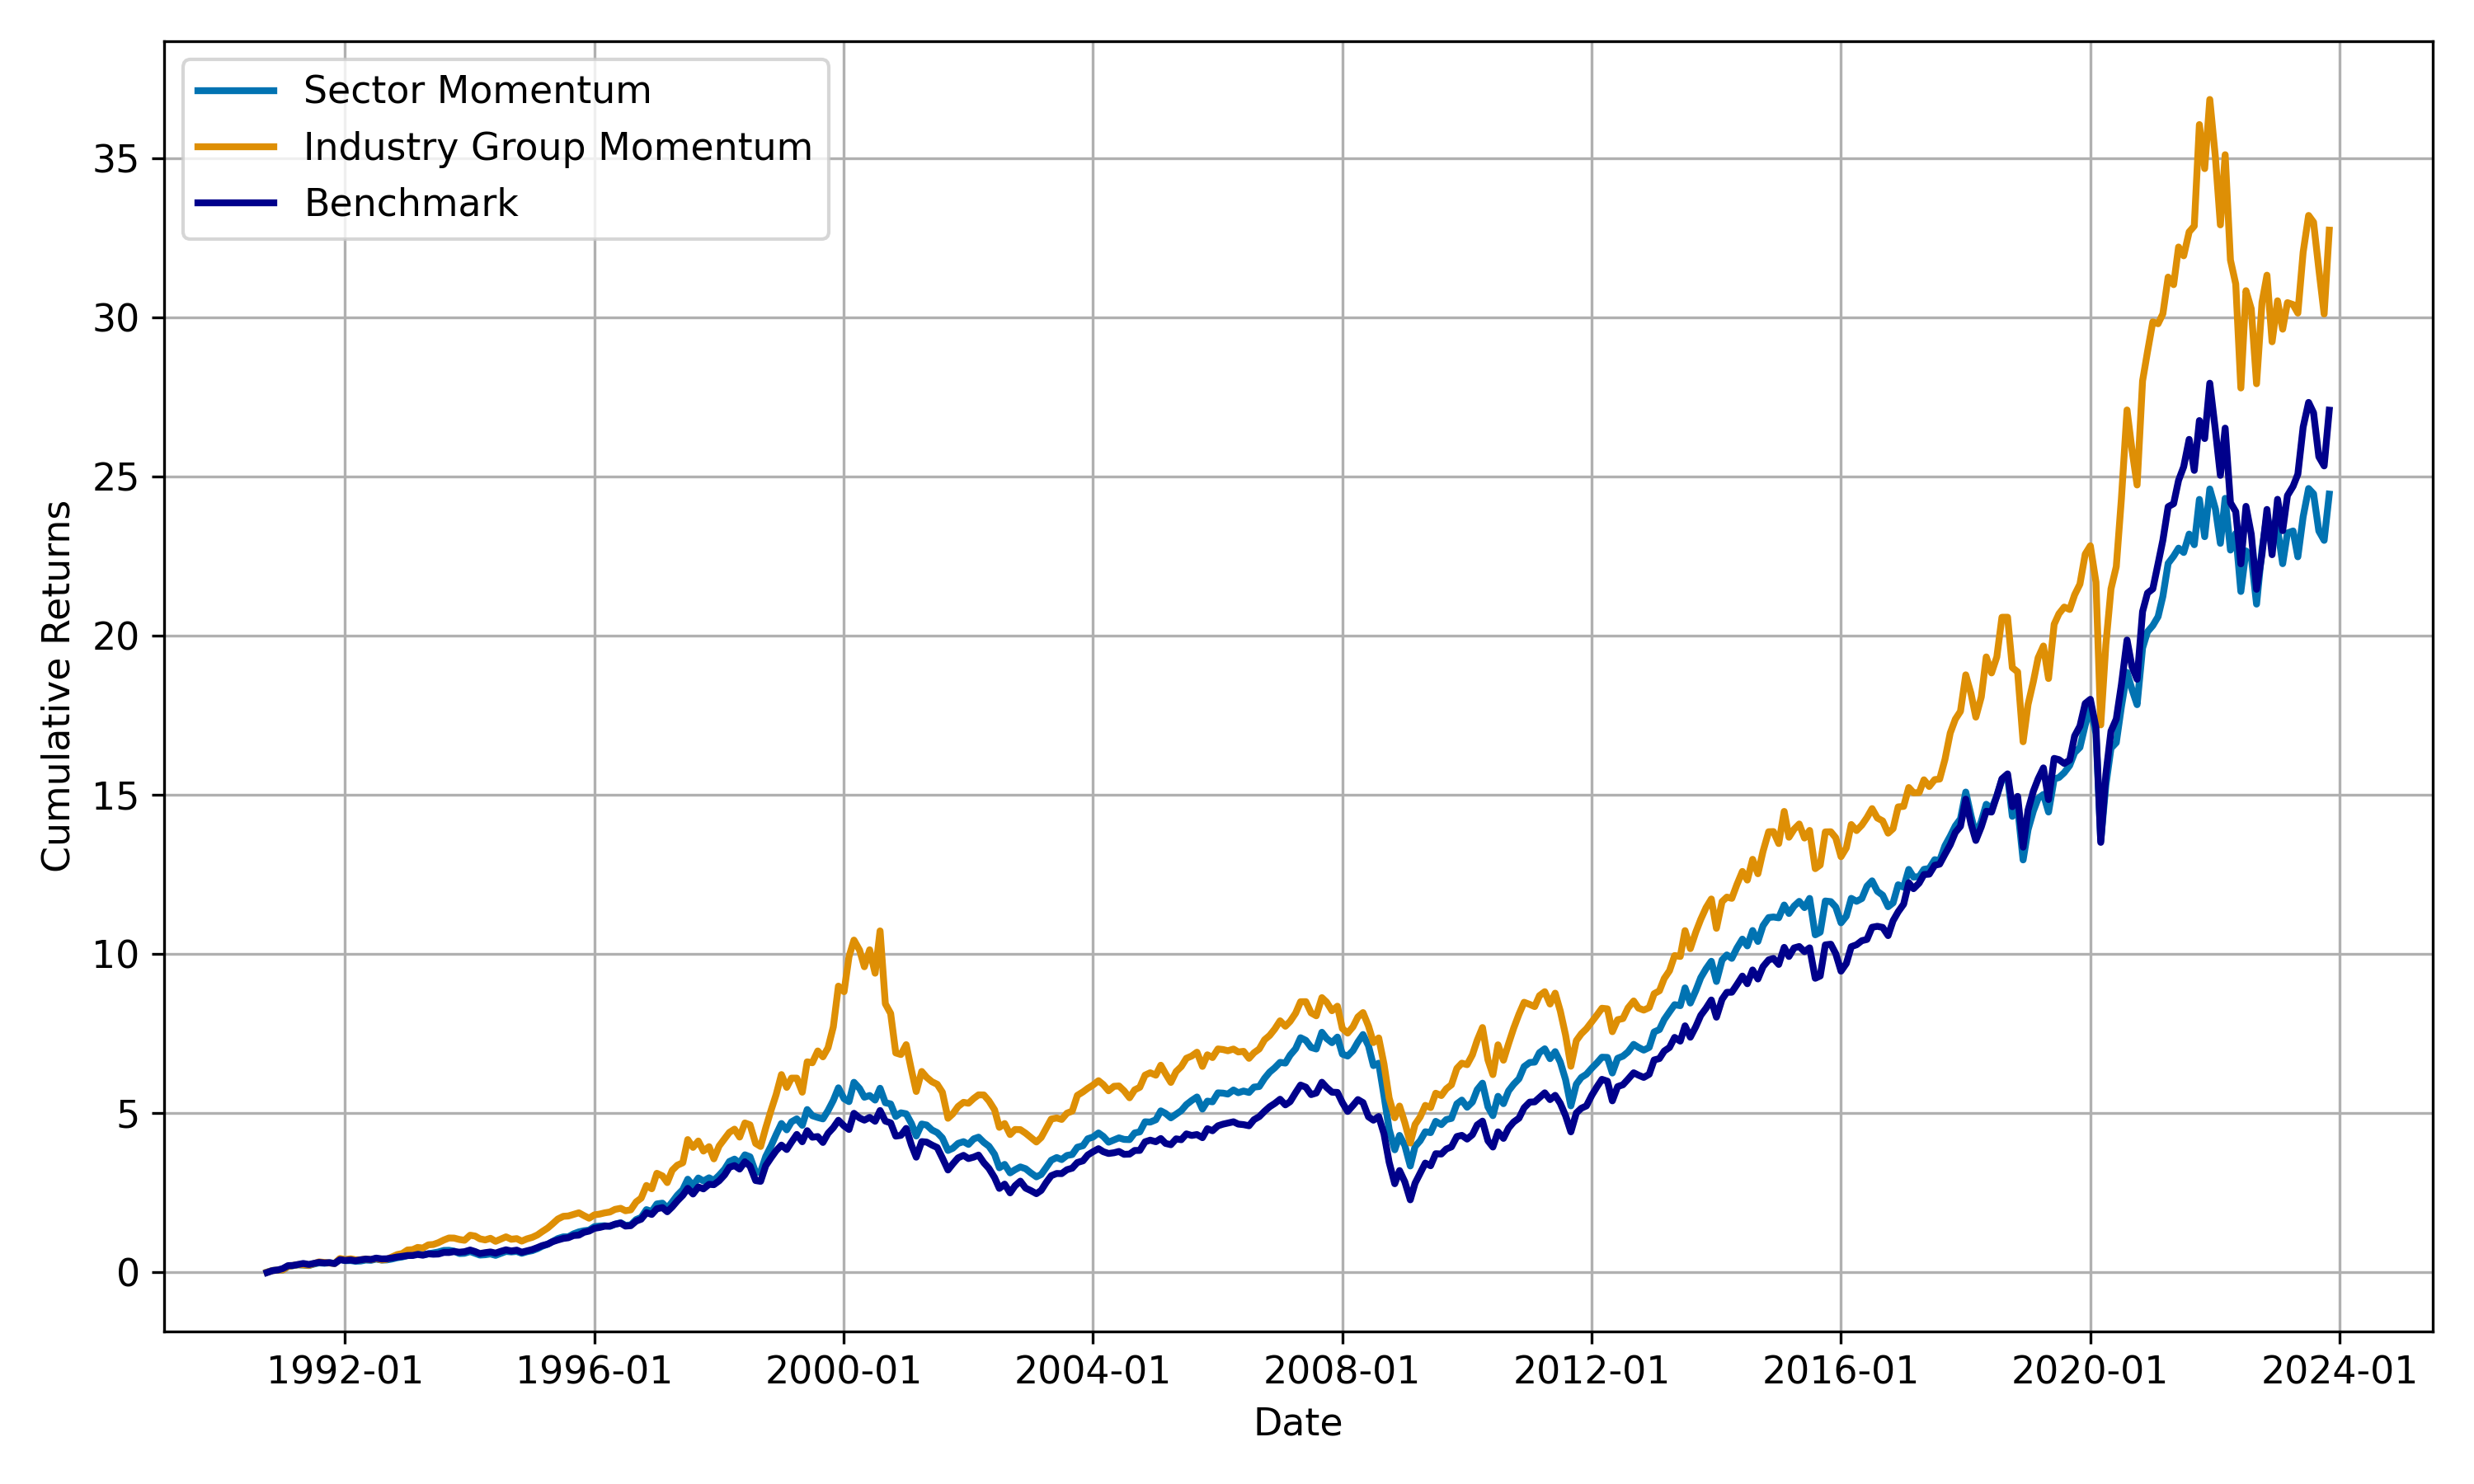
\includegraphics[width=1\textwidth]{Plots/strategy_plot.png}}
\end{figure}

\newpage
We then explored whether the momentum strategy is only effective in a long only setup or if incorporating a short component could add value. The short setups showed significantly lower returns compared to the risk-free rate. The underperformance, coupled with higher volatility, renders the strategy unattractive from a risk-return perspective (see \textit{Table \ref{tab_02}} and \textit{Figure \ref{fig_02}}).

One of the key reasons for this outcome is the occurrence of momentum crashes as often cited in literature. These crashes significantly affect long/short strategies, as the short positions, which had been underperforming, suddenly exhibit abnormal gains, thus undermining the overall strategy performance. 

Similarly to long only portfolios weights for long/short are balanced for sector portfolios and more spread out with increased number of constituents for industry group portfolios (see \textit{Figure \ref{fig_12}} and \textit{Figure \ref{fig_13}}). 

\begin{figure}[H] 
        \caption{Long/Short Momentum Performance vs.~Risk Free Rate} 
    \label{fig_02}
    \textit{Figure \ref{fig_02}} displays net cumulative returns for long only and long/short sector and industry group momentum portfolios from October 1990 to October 2023. The portfolios, with a 3-month holding period and a 9-month lookback period, are rebalanced monthly to take long (short) positions in the best (worst) performing sectors/industry groups of the market-weighted S\&P 500. Proportional transaction costs of 10 basis points are assumed.
    
\captionsetup{justification=centering}
\centerline{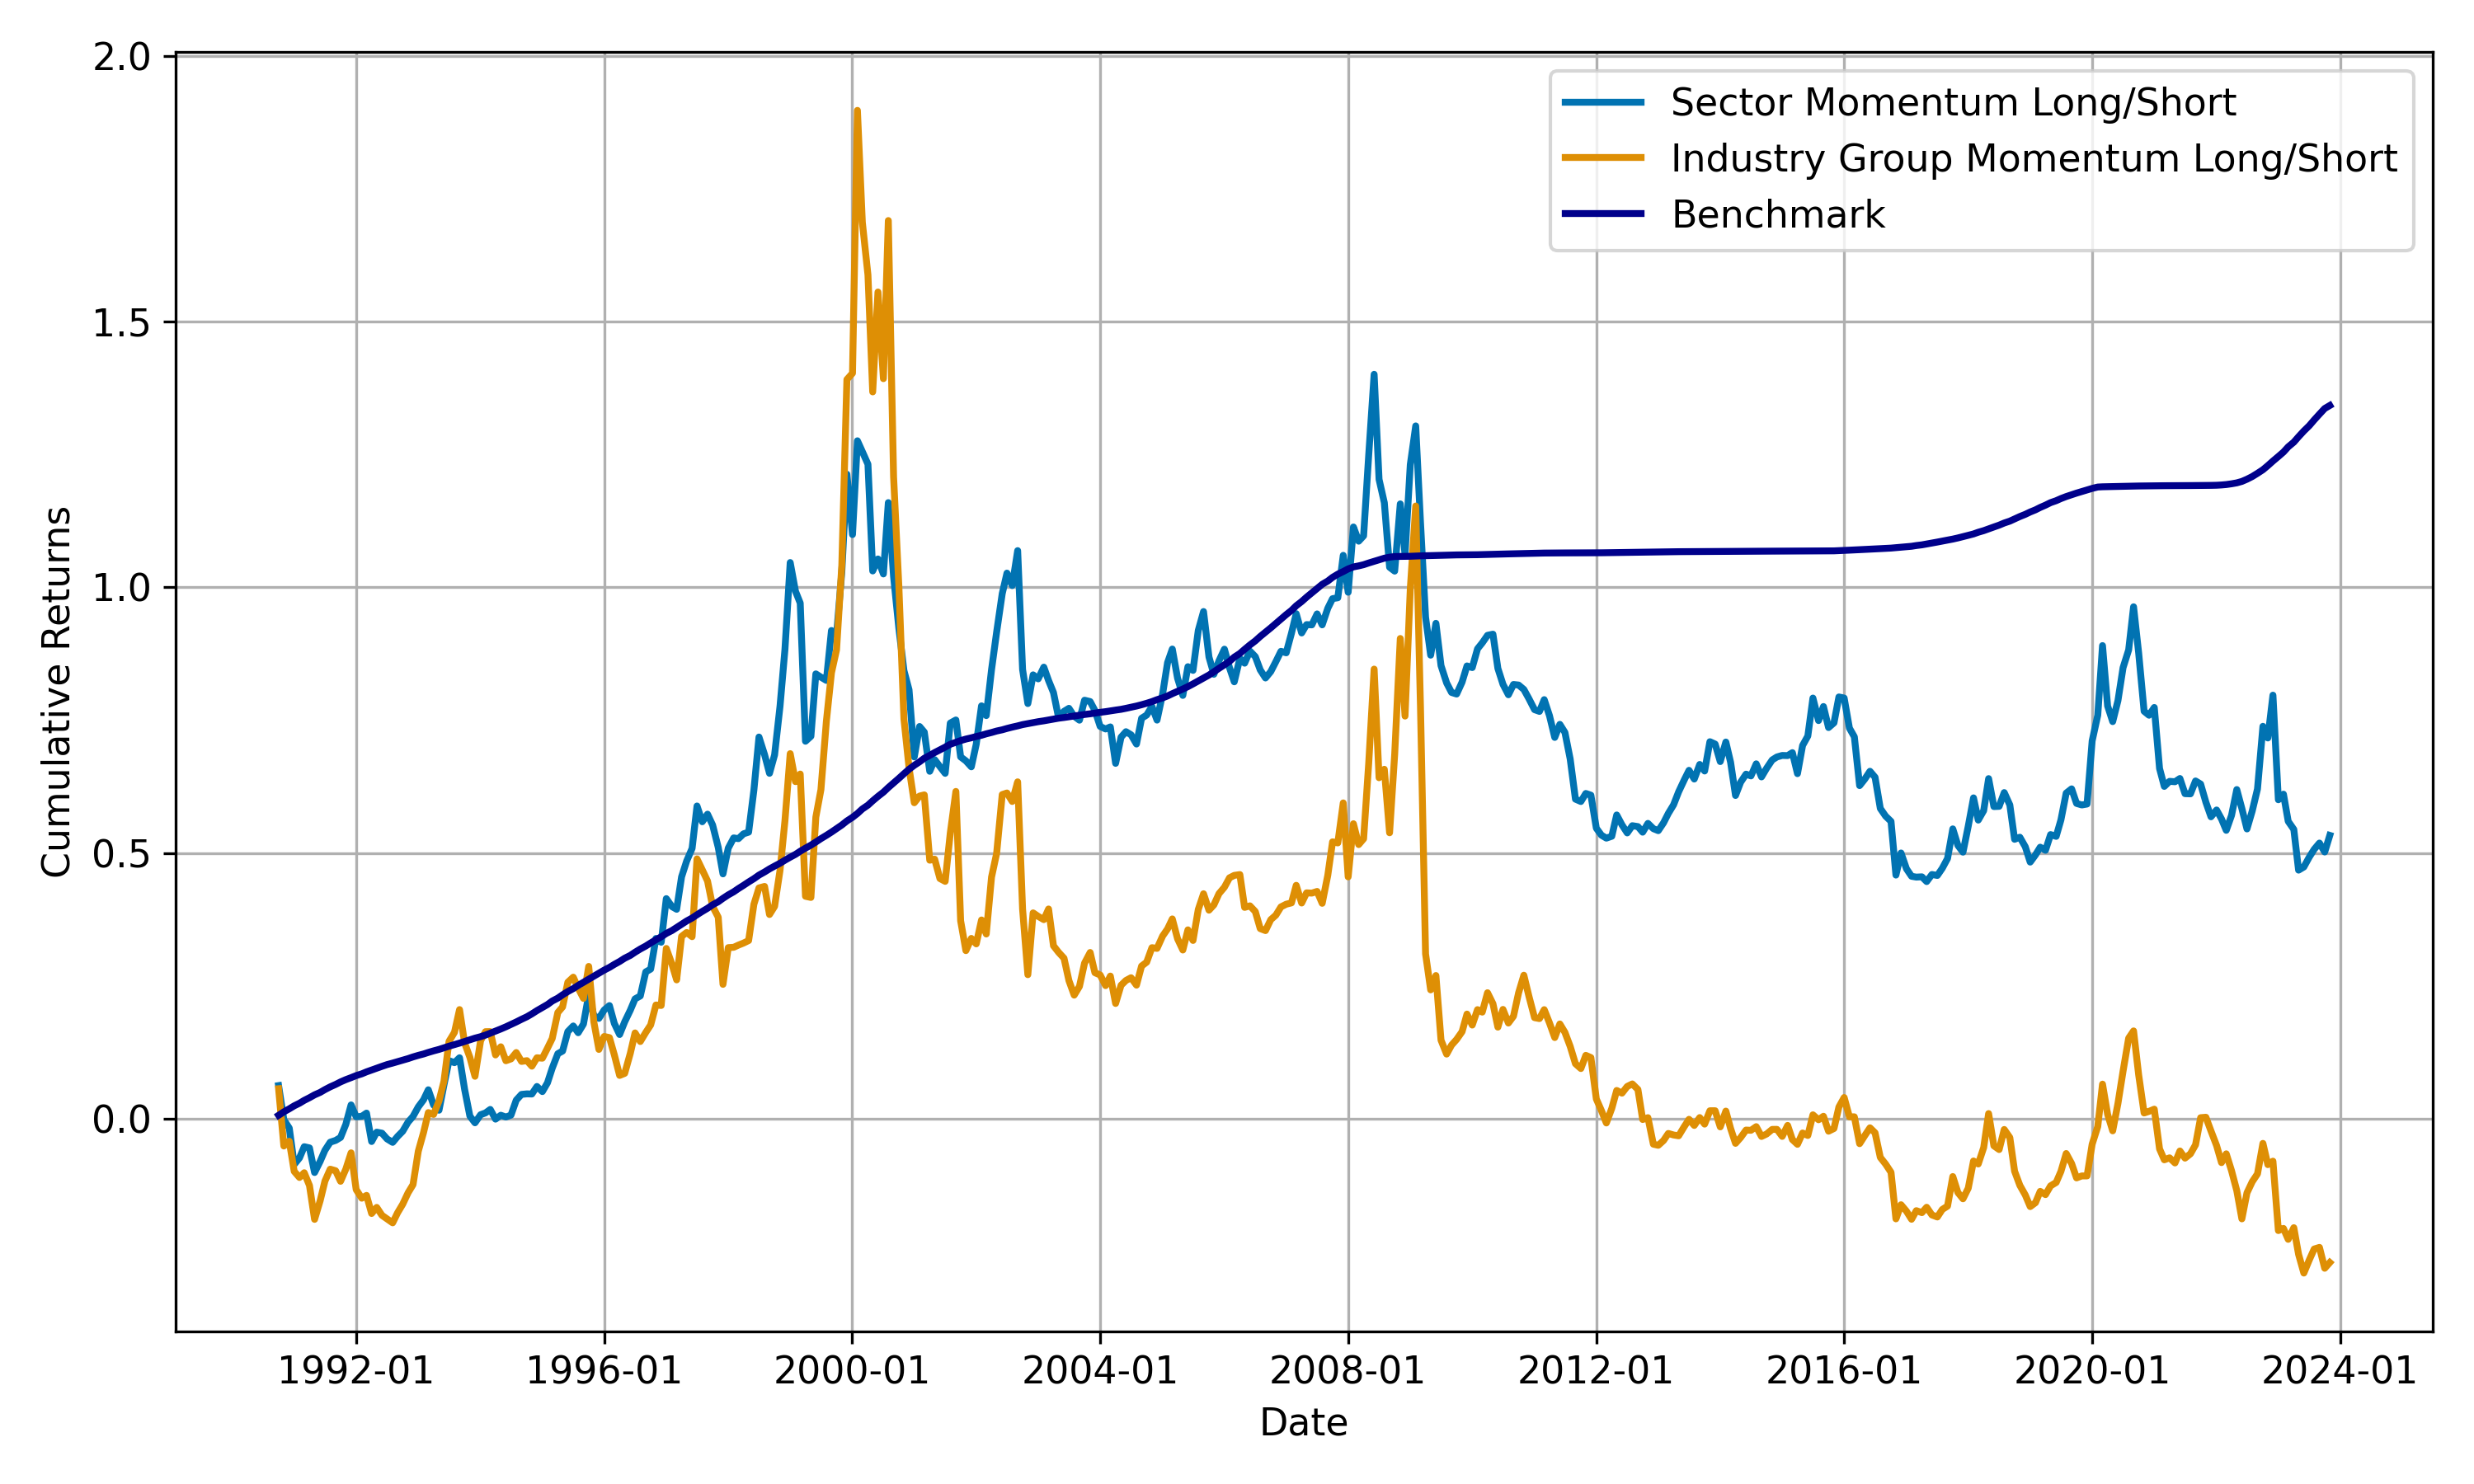
\includegraphics[width=1\textwidth]{Plots/strategy_plot_long_short.png}}
\end{figure}

\newpage
\section{Robustness checks}
We explore further implementation possibilities of our long only strategy by varying the lookback period, holding period, number of holdings and transaction costs. 

When analyzing the relationship between Sharpe Ratios and the lookback period (see \textit{Figure \ref{fig_06}}), we observe that Sharpe Ratios seem to decline with longer lookback horizons somehow challenging the findings of \cite{jegadeesh1993returns} who found the highest return for a lookback period of 9 months. 

\begin{figure}[H]
        \captionsetup{justification=centering}
   \caption{Net Sharpe Ratios vs.~Lookback Period for Long Only Sector and Industry Group Momentum Portfolios}
    \label{fig_06}
        \textit{Figure \ref{fig_06}} reports net Sharpe Ratios for long only sector and industry group momentum portfolios with a holding period of 3 months whereby the monthly rebalanced portfolio takes long positions in the 3 best performing sectors/industry. Proportional transaction costs of 10 basis points are assumed. The figure shows results for the period between October 1990 to October 2023. The x-axis represents the lookback period which can take values between 1 to 12 months.
    \centerline{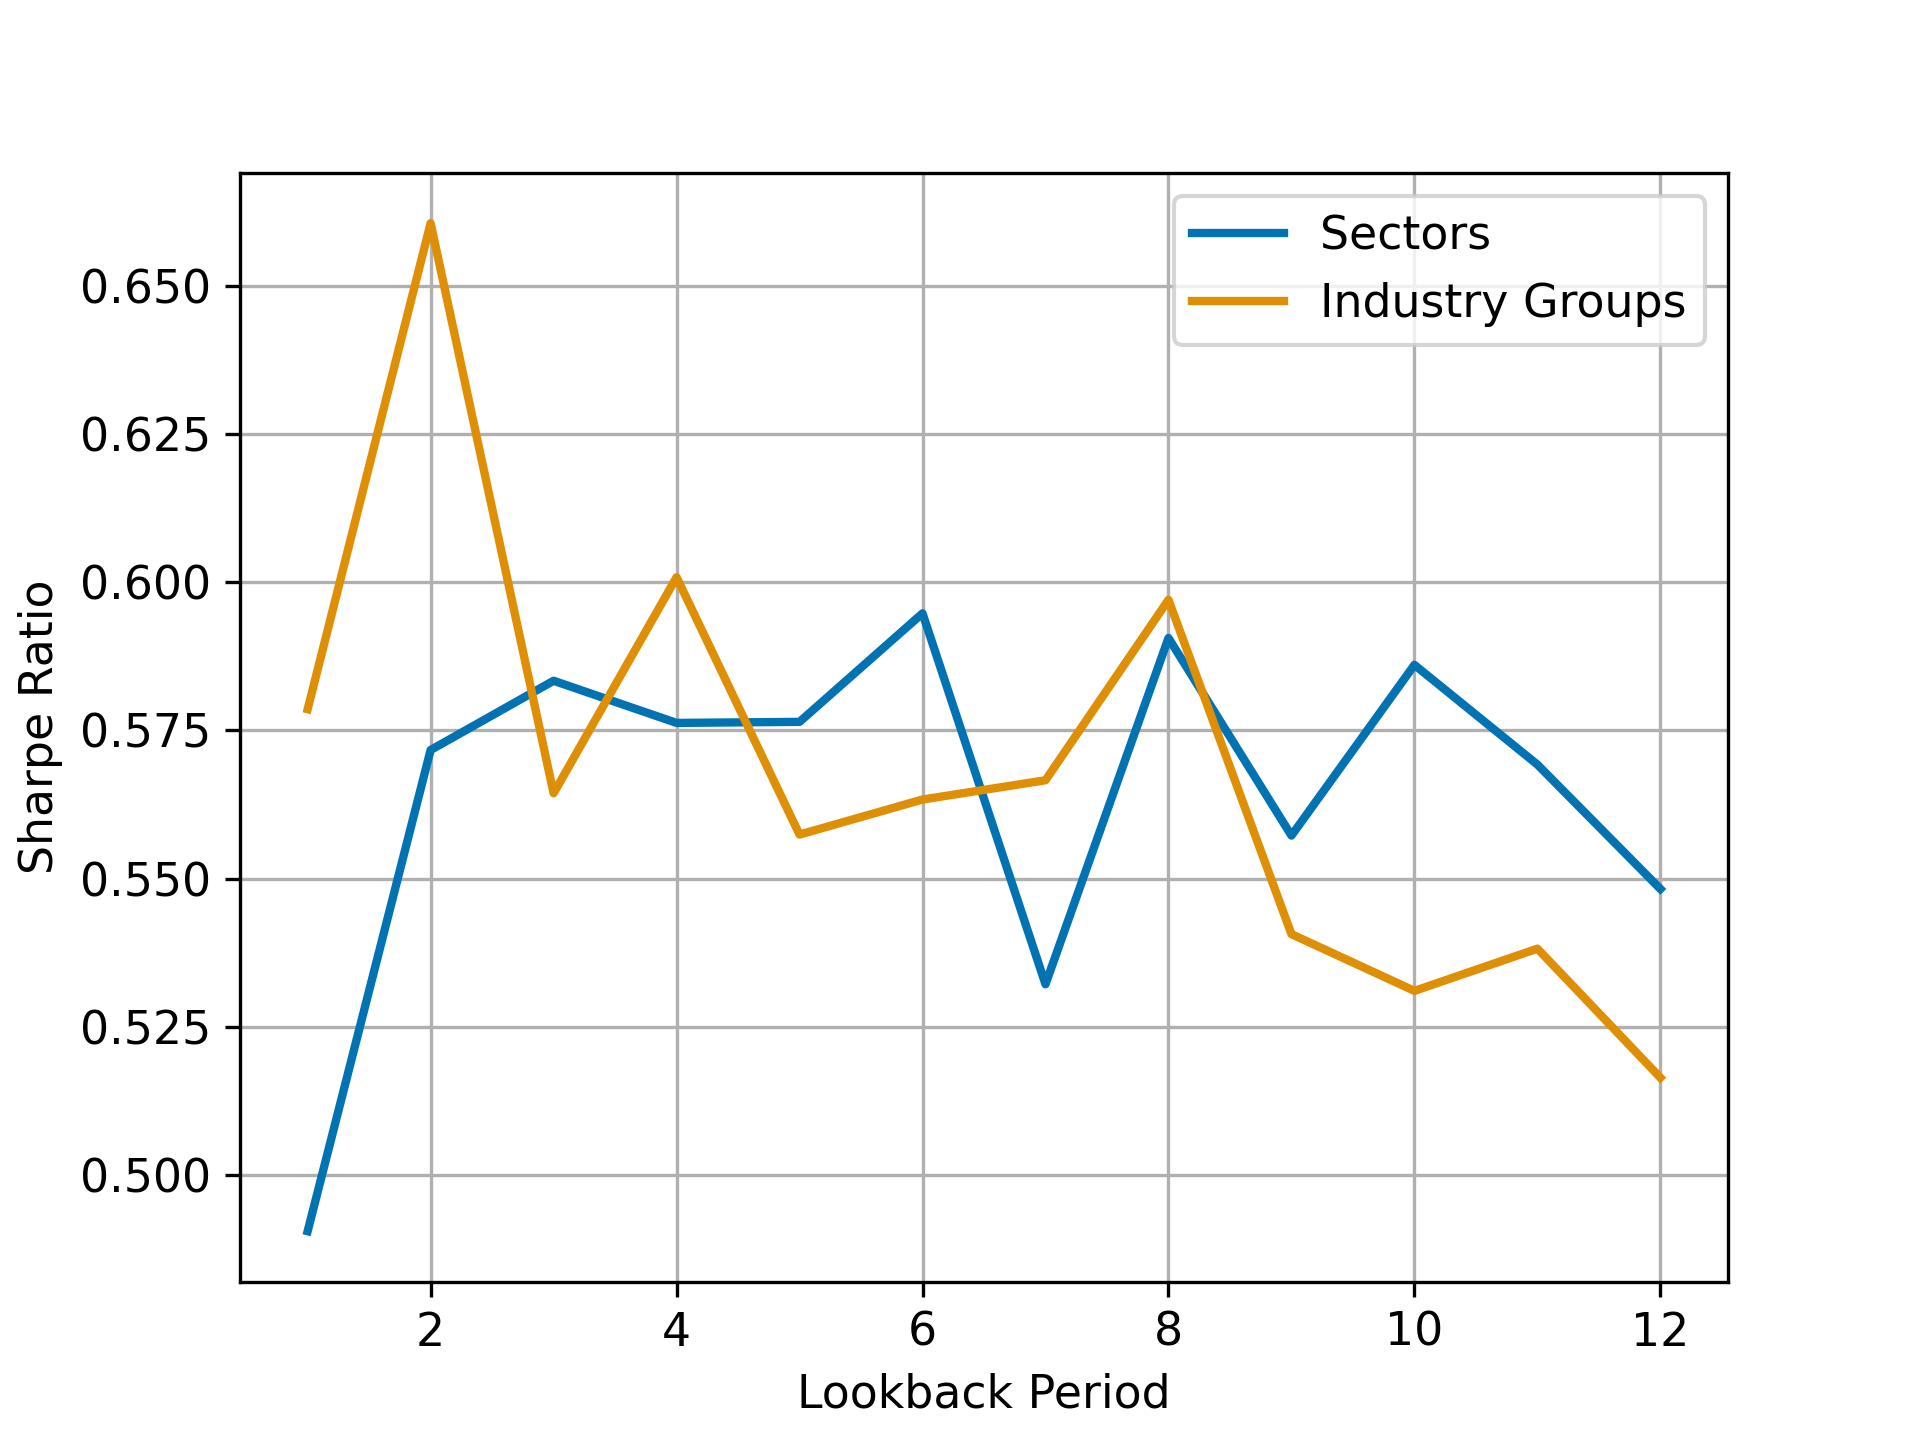
\includegraphics[width=1\textwidth]{Plots/robustness_check_lookback.png}}
\end{figure}

\newpage
Secondly, we analyze the relationship between Sharpe Ratios and the holding period (see \textit{Figure \ref{fig_05}}). There seems to be no clear relation between the holding period and the Sharpe Ratios. Generally, this boils down to autocorrelation in returns. Intuitively one would assume that autocorrelations of returns decline with longer investment horizons, something we cannot observe in our robustness check at hand.

\begin{figure}[H]
       \captionsetup{justification=centering}
   \caption{Net Sharpe Ratios vs.~Holding Period for Long Only Sector and Industry Group Momentum Portfolios}
    \label{fig_05}
        \textit{Figure \ref{fig_05}} reports net Sharpe Ratios for long only sector and industry group momentum portfolios with a lookback period of 9 months whereby the monthly rebalanced portfolio takes long positions in the 3 best performing sectors/industry groups of the market-weighted S\&P500. Proportional transaction costs of 10 basis points are assumed. The figure shows results for the period between October 1990 to October 2023. The x-axis represents the holding period which can take values between 1 to 12 months.
    \centerline{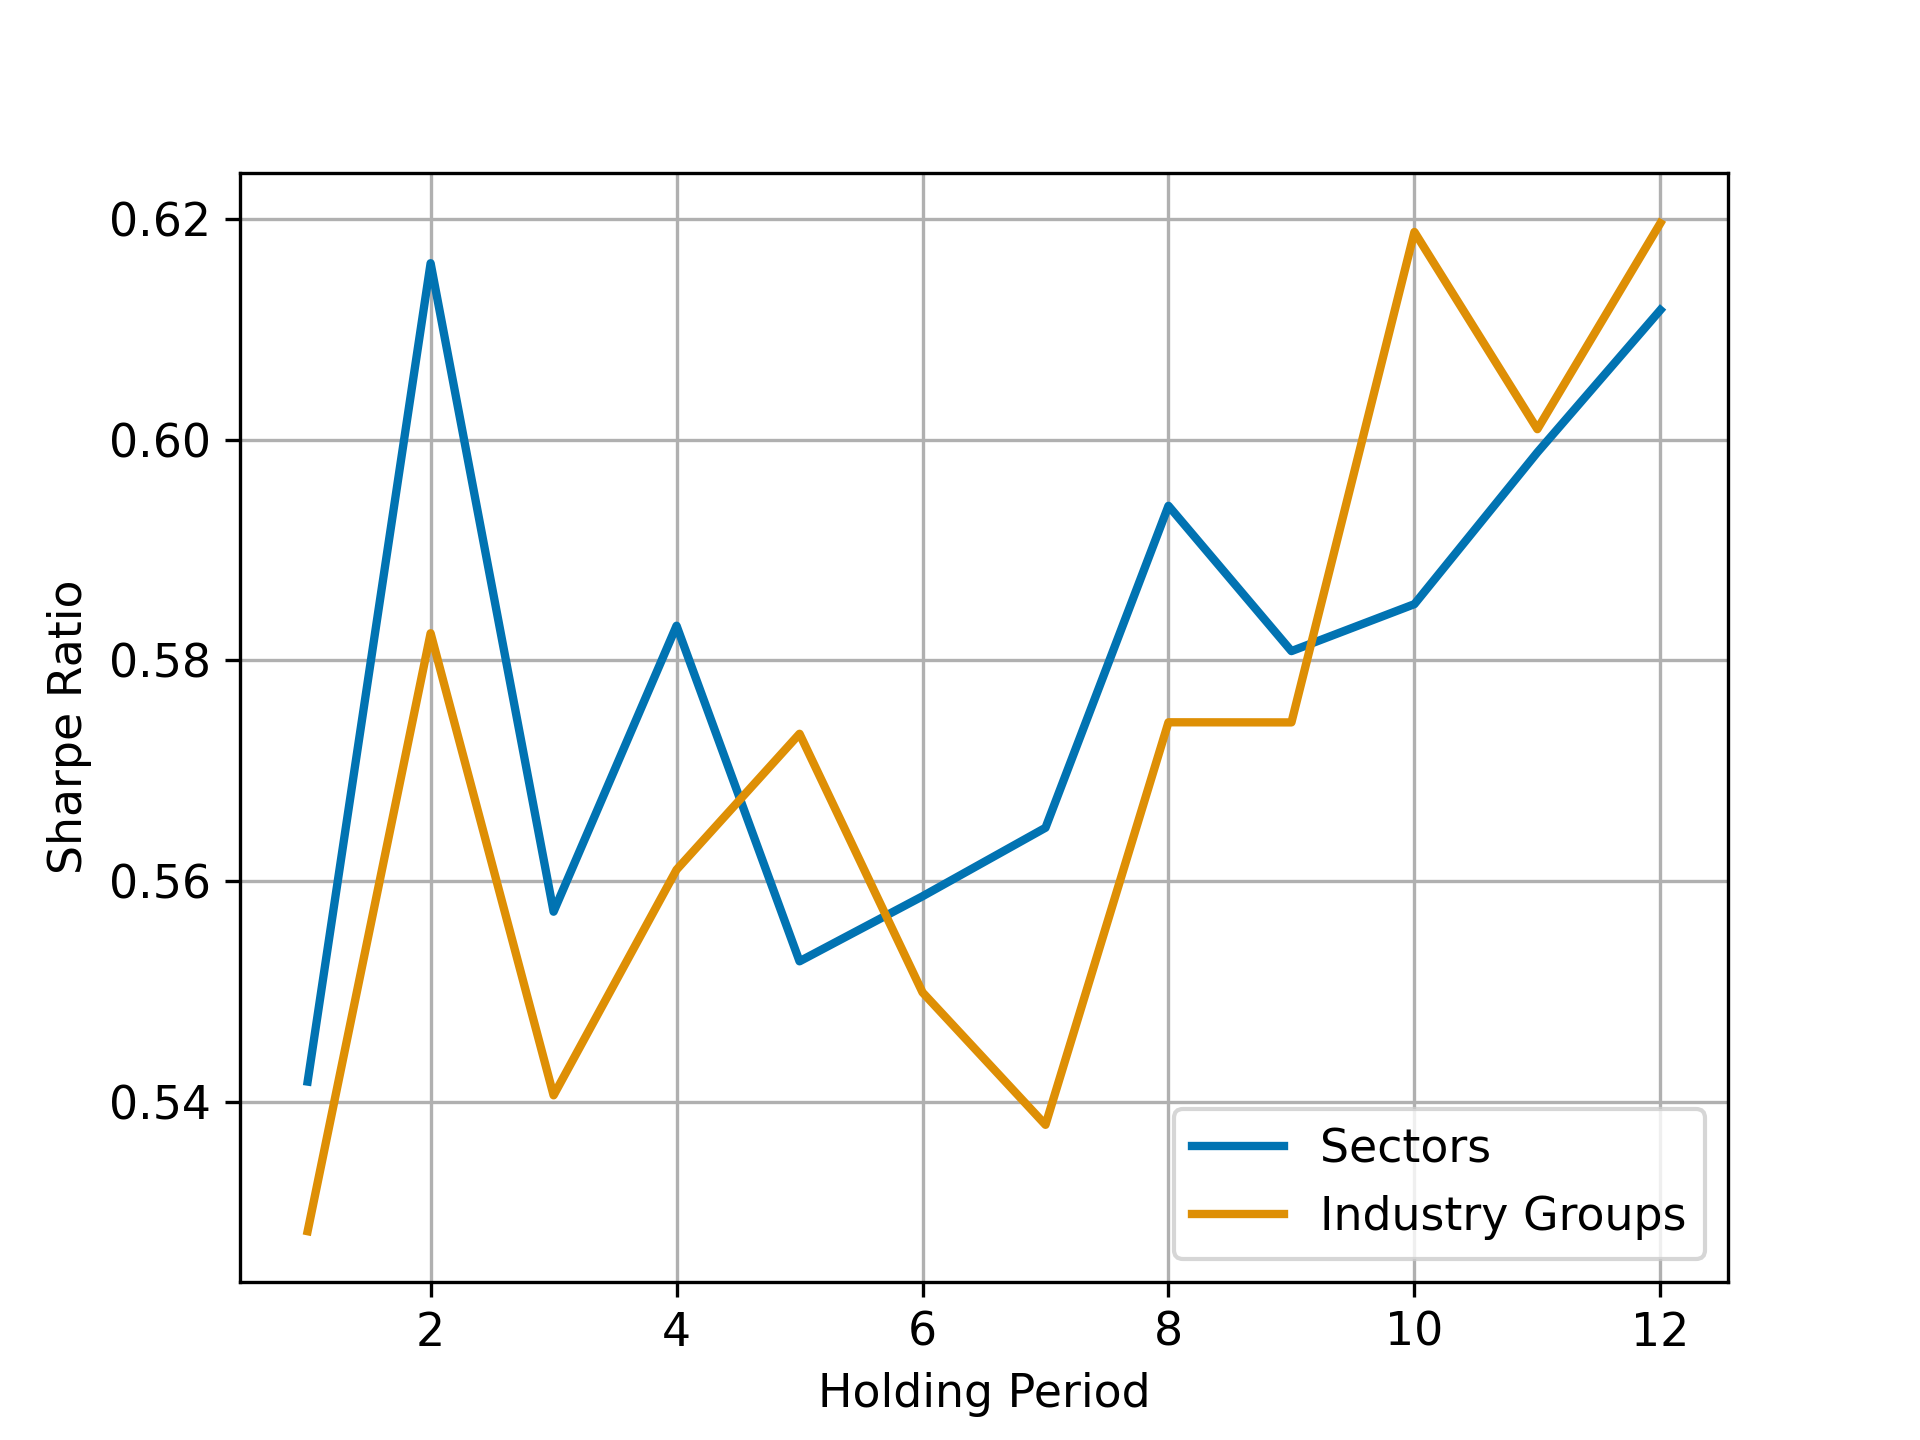
\includegraphics[width=1\textwidth]{Plots/robustness_check_holdingperiod.png}}
\end{figure}

\newpage
Next, we analyze the relationship between number of holdings and Sharpe Ratios (see \textit{Figure \ref{fig_04}}). We find that that increasing the number of holdings seems to improve Sharpe Ratios most likely because of the reduced volatility due to diversification which is in line with most academic literature.\\


\begin{figure}[H] 
       \captionsetup{justification=centering}
    \caption{Net Sharpe Ratios vs.~Number of Holdings for Long Only Sector and Industry Group Momentum Portfolios} 
    \label{fig_04}
        \textit{Figure \ref{fig_04}} displays net Sharpe Ratios returns for long only sector and industry group momentum portfolios from October 1990 to October 2023. The portfolios, with a 3-month holding period and a 9-month lookback period, are rebalanced monthly to take long positions in the best performing sectors/industry groups of the market-weighted S\&P 500. We assumed transaction costs of 10 basis points. The x-axis represents the number of holdings which can take values between 1 to 5.
    \centerline{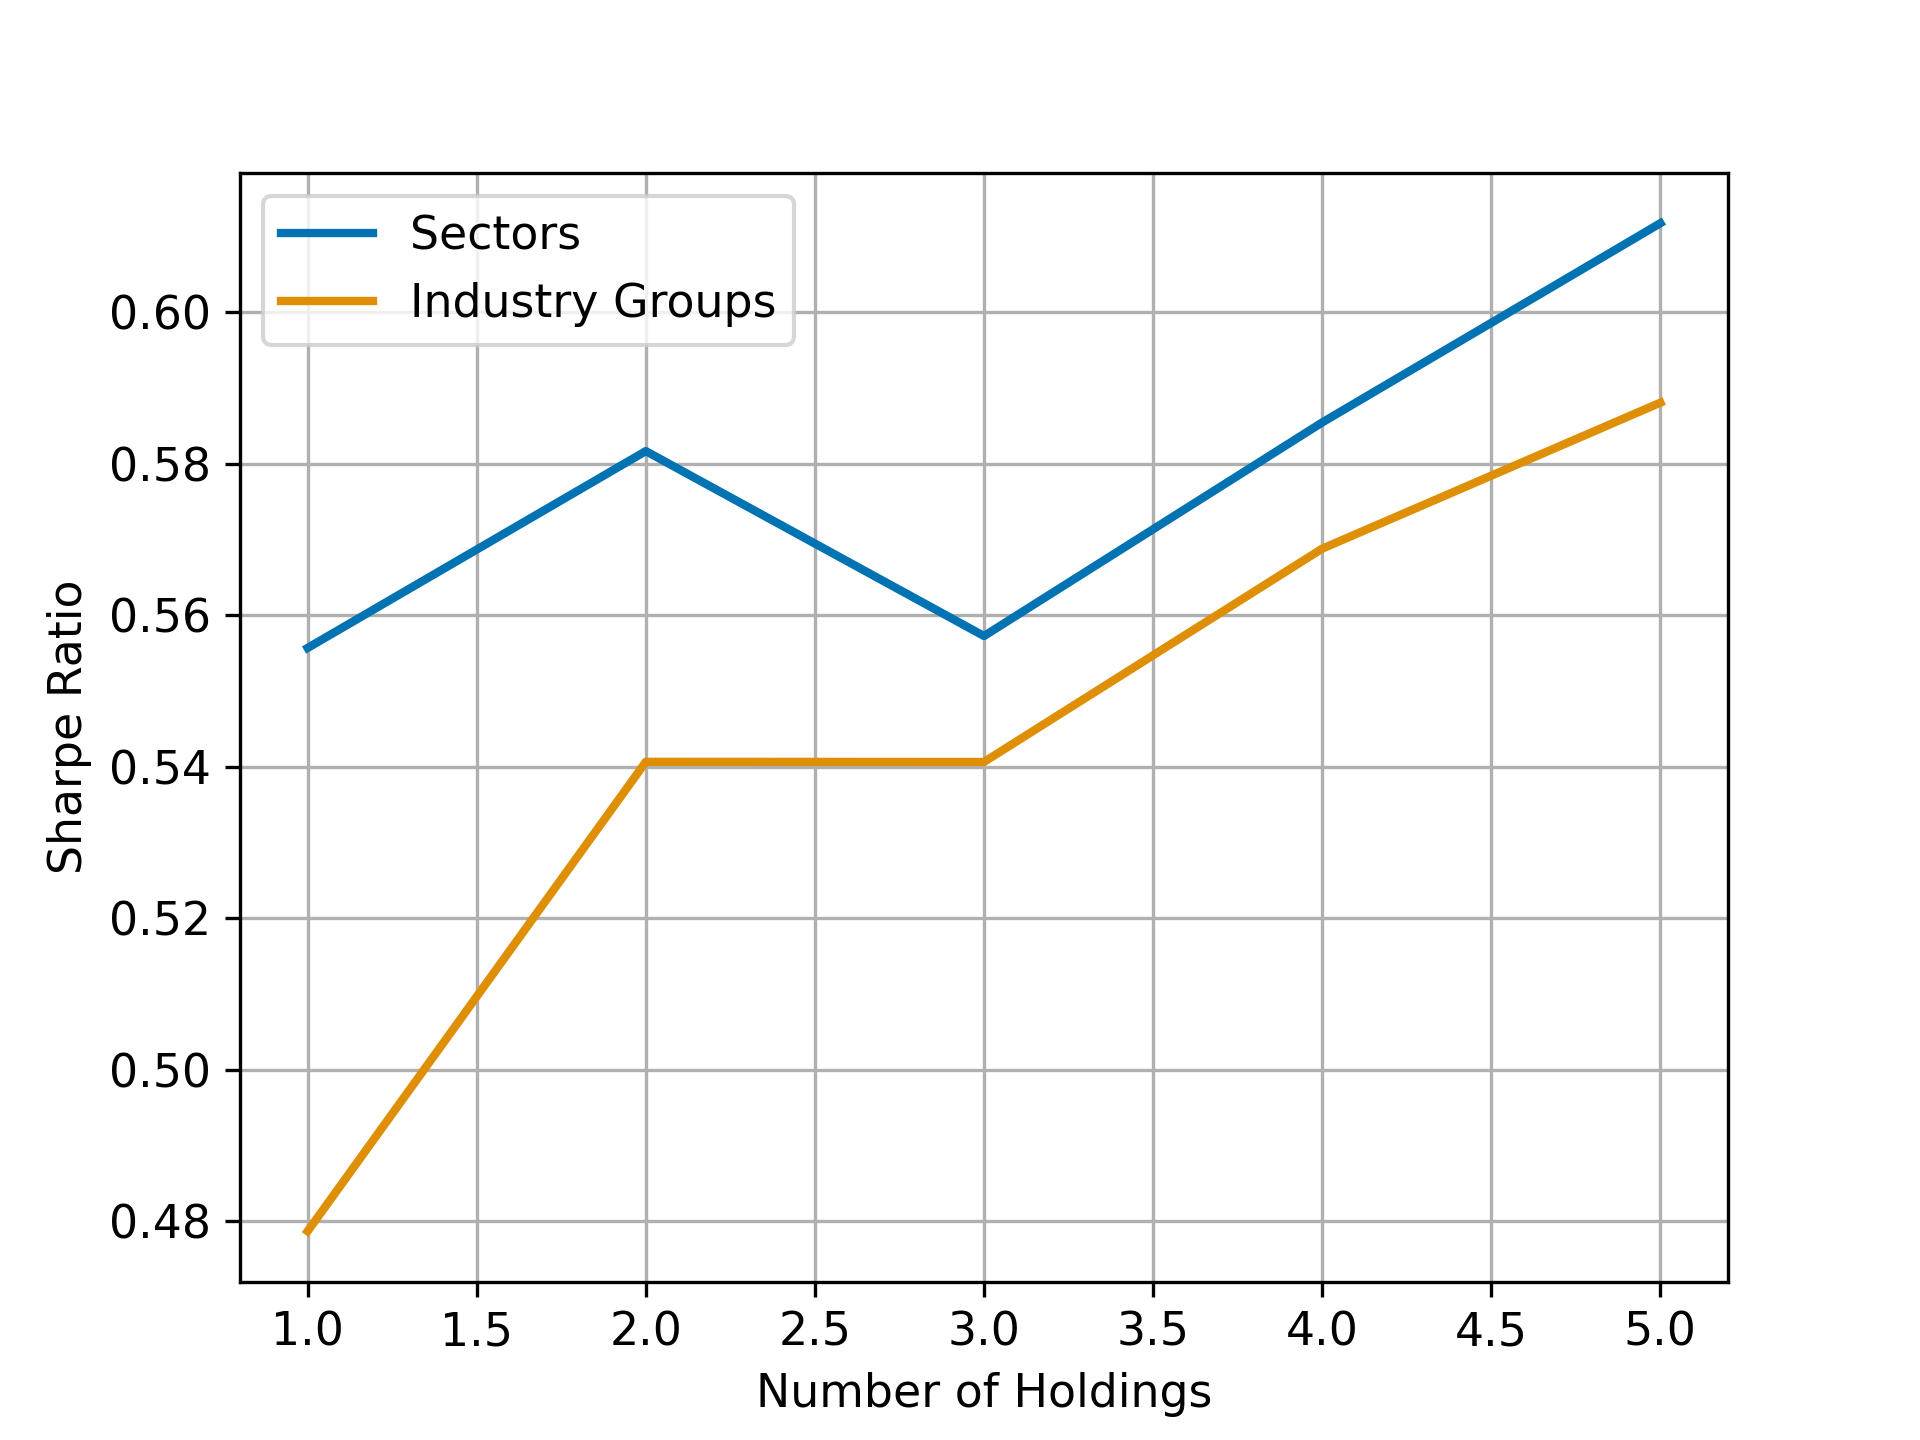
\includegraphics[width=1\textwidth]{Plots/robustness_check_holdings.png}}
\end{figure}


\newpage
Furthermore, given the original motivation to build implementable, i.e. profitable momentum strategies after transaction costs, we analyze the profitability of the long only momentum implementation for varying degrees of transaction costs (see \textit{Figure \ref{fig_03}}). Since only industry group implementations seem to work, we only focused on industry groups in this part. We find that the long only momentum strategy is profitable up to 25 basis points proportional transaction cost whereby the strategy is therefore also profitable with 10 basis points proportional transaction cost as previously shown.\\

\begin{figure}[H]
           \captionsetup{justification=centering}
   \caption{Net Performance vs.~Level of Transaction Costs for Long Only Industry Group Momentum Portfolios}
    \label{fig_03}
    \textit{Figure \ref{fig_03}} displays net cumulative returns for long only industry group momentum portfolios with a holding period of 3 months and a lookback period of 9 months whereby the monthly rebalanced portfolio takes long positions in the 3 best performing sectors of the market-weighted S\&P500. The figure shows results for the period between October 1990 to October 2023. Different line colors represent different proportional transaction costs ranging from 10 to 100 basis points.
    \centerline{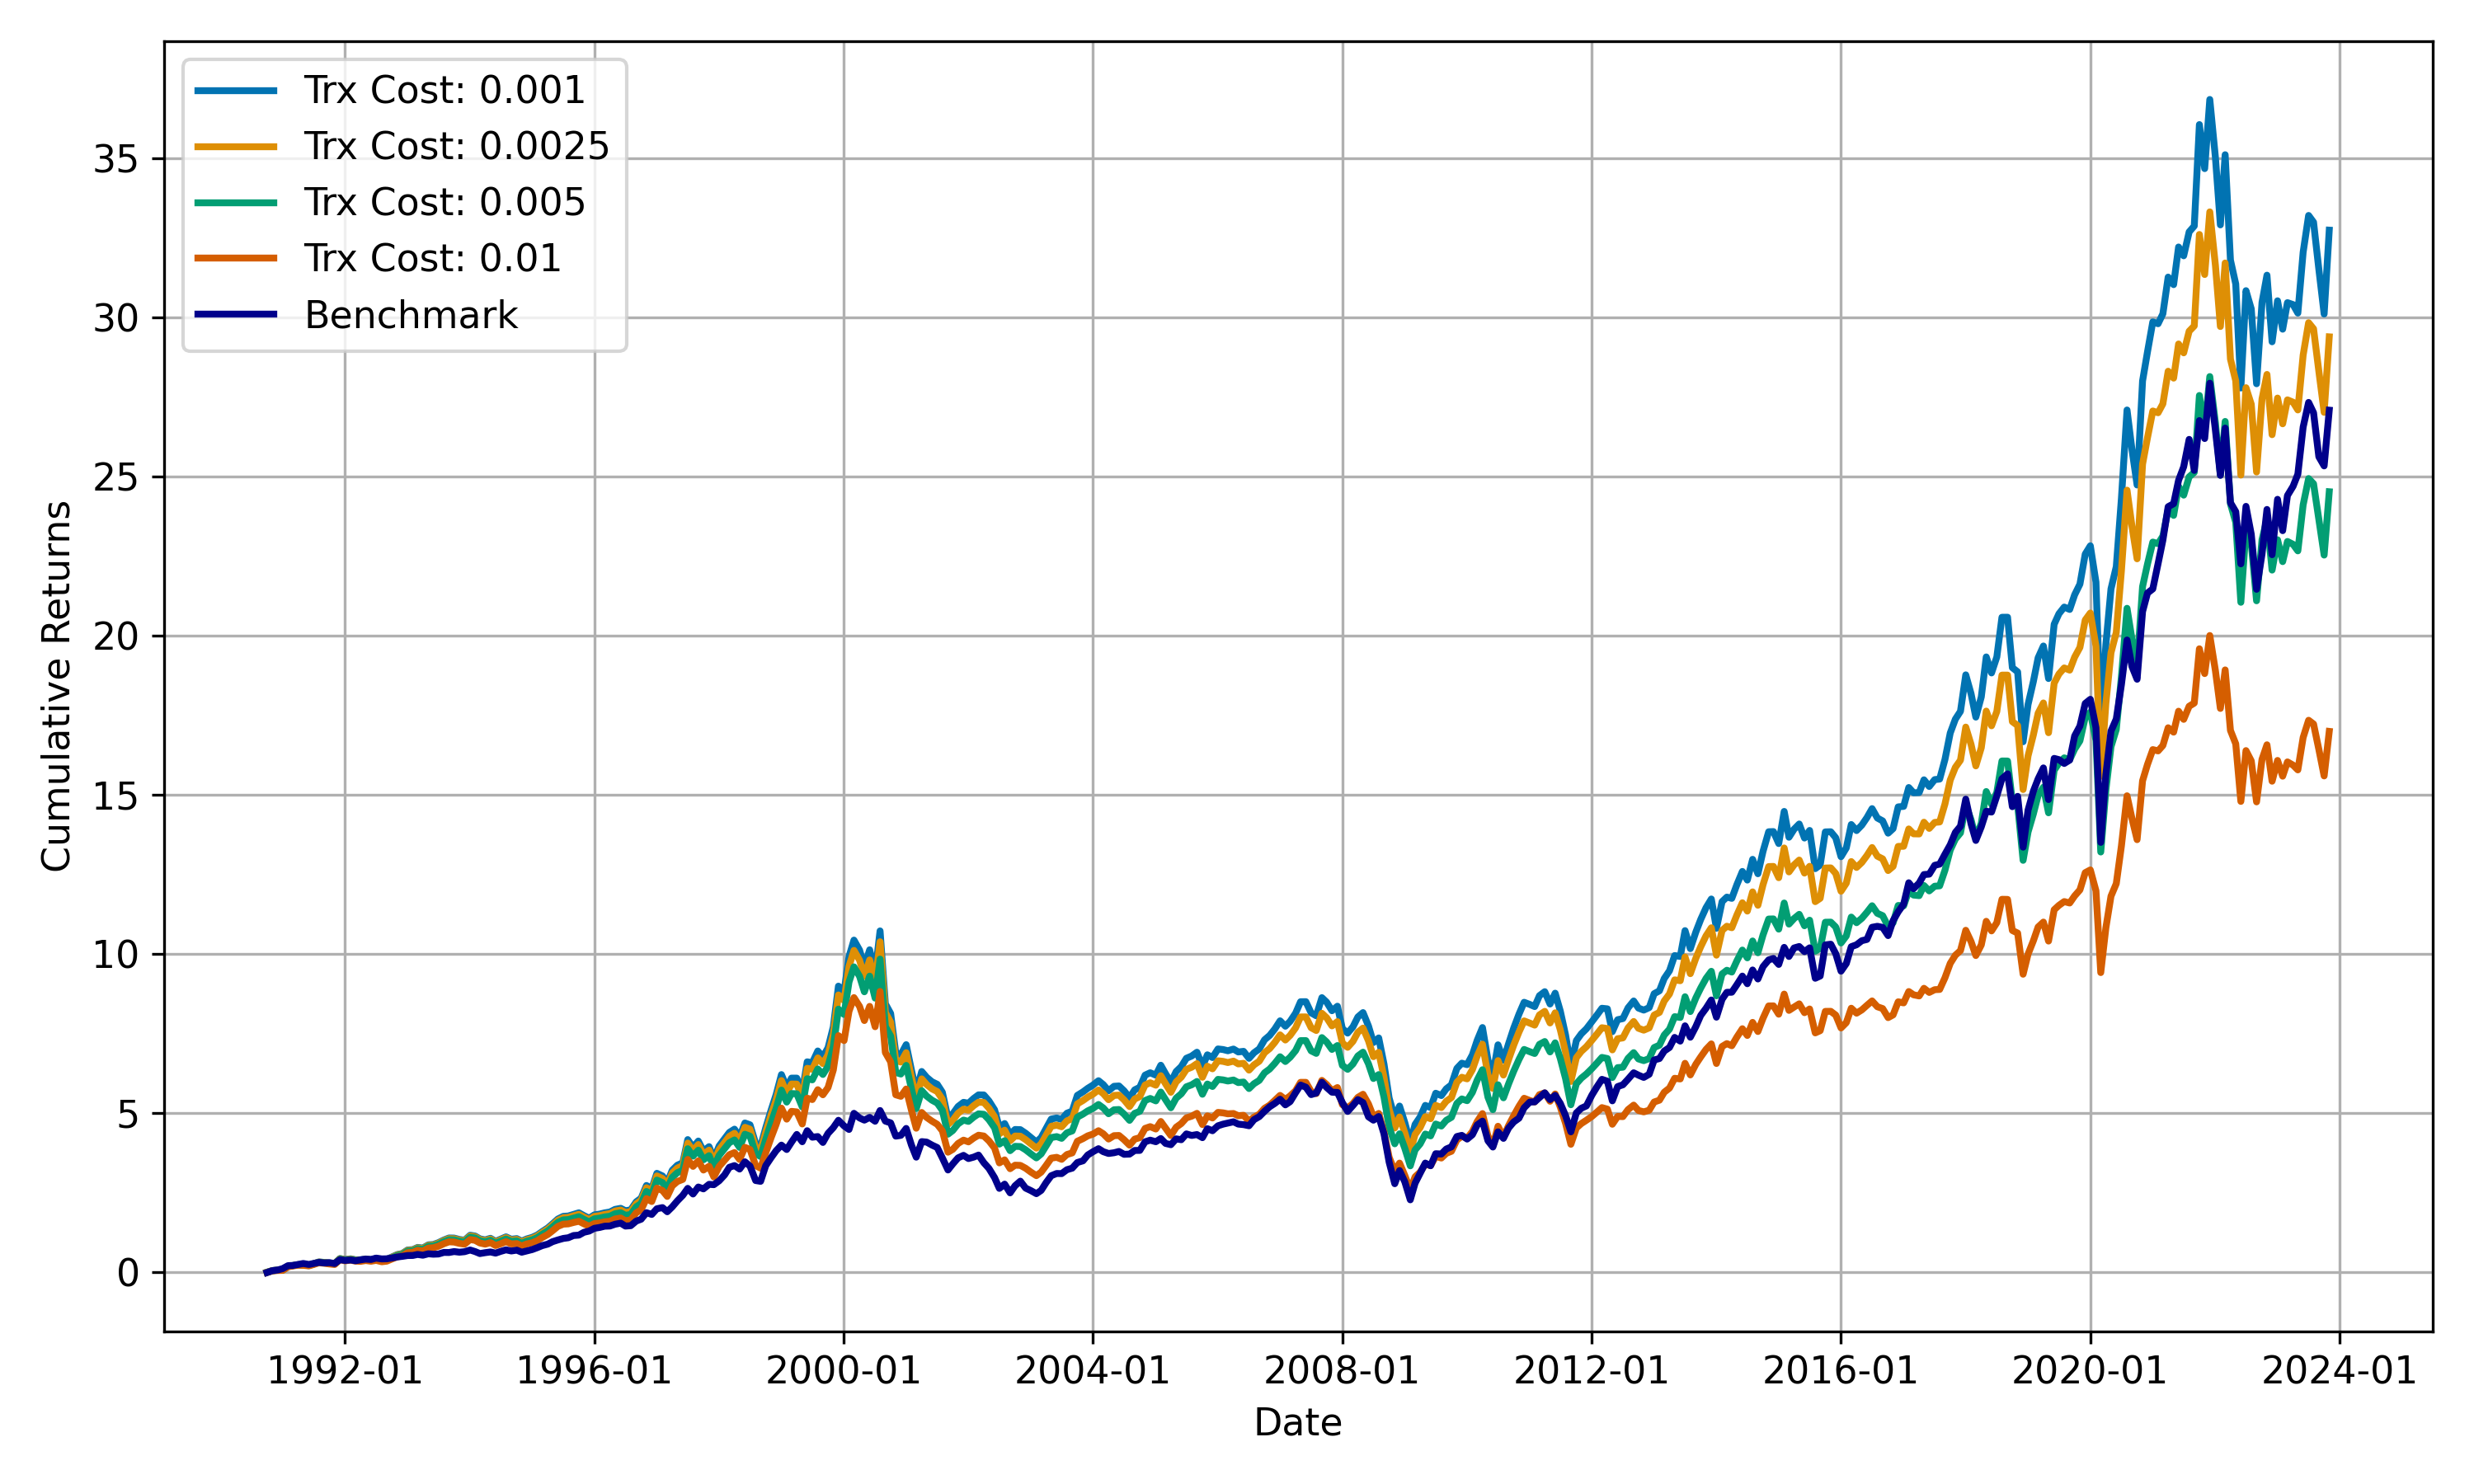
\includegraphics[width=1\textwidth]{Plots/robustness_check_tc.png}}
\end{figure} 

\newpage
\section{Conclusion}
    Our research investigates the performance and robustness of sector and industry group momentum investment strategies. We analyzed these strategies both in isolation and in combination and examined for robustness of various portfolio parameters such as the holding period, lookback period, the number of holdings, as well as transaction costs.\\

    Our results confirm that momentum investment strategies, particularly those incorporating an industry group rotation approach, can deliver excess returns consistent with the broader academic and empirical evidence. We find that pure momentum strategies, especially the long-only strategy, generate outperformance. However, the inclusion of a short leg negatively impacts momentum strategies due to the negative impact of momentum crashes. On a sector level, however, momentum does not seem to work probably because reducing the universe to 11 constituents takes away too much flexibility in picking trending parts of the markets and therefore, equalizes the returns more in line with the overall market.\\

    As a takeaway we would say that momentum strategies can indeed be interesting strategies to be implemented in a portfolio context. However, the universe to select from plays a crucial role and is arguably more important than other input parameters such as lookback period or investment horizon.\\


\newpage
\bibliographystyle{plainnat}
\bibliography{biblio}

\renewcommand{\thesection}{A}
\section{Appendix}
\subsection{Data table}

\begin{table}[H]
\caption{Bloomberg Data}
    The table presents the downloaded data from Bloomberg. Used data is risk free, total return S\&P500 sector and industry group indices as well as the total return S\&P500. Daily data is used since inception of the sector and industry group indices. Fields are RT116 (TOT\_RETURN\_INDEX\_GROSS\_DVDS) and PR005 (PX\_LAST).
\begin{tabular}{@{\extracolsep{12pt}} lccc}
\\[-1.8ex]\hline
\hline \\[-1.8ex]
Bloomberg Ticker & Bloomberg Field & Frequency & Time Horizon \\ 
\hline \\[-1.8ex]
GB03 Govt & PR005 & Daily & 12.09.1989 - 17.11.2023 \\
S5AUCO Index & RT116 & Daily & 12.09.1989 - 17.11.2023 \\
S5BANKX Index & RT116 & Daily & 12.09.1989 - 17.11.2023 \\
S5COMS Index & RT116 & Daily & 12.09.1989 - 17.11.2023 \\
S5COND Index & RT116 & Daily & 12.09.1989 - 17.11.2023 \\
S5CONS Index & RT116 & Daily & 12.09.1989 - 17.11.2023 \\
S5CPGS Index & RT116 & Daily & 12.09.1989 - 17.11.2023 \\
S5DIVF Index & RT116 & Daily & 12.09.1989 - 17.11.2023 \\
S5ENRS Index & RT116 & Daily & 12.09.1989 - 17.11.2023 \\
S5ENRSX Index & RT116 & Daily & 12.09.1989 - 17.11.2023 \\
S5FDBT Index & RT116 & Daily & 12.09.1989 - 17.11.2023 \\
S5FINL Index & RT116 & Daily & 12.09.1989 - 17.11.2023 \\
S5FDSR Index & RT116 & Daily & 12.09.1989 - 17.11.2023 \\
S5HCES Index & RT116 & Daily & 12.09.1989 - 17.11.2023 \\
S5HLTH Index & RT116 & Daily & 12.09.1989 - 17.11.2023 \\
S5HOUS Index & RT116 & Daily & 12.09.1989 - 17.11.2023 \\
S5HOTR Index & RT116 & Daily & 12.09.1989 - 17.11.2023 \\
S5INDU Index & RT116 & Daily & 12.09.1989 - 17.11.2023 \\
S5INFT Index & RT116 & Daily & 12.09.1989 - 17.11.2023 \\
S5INSU Index & RT116 & Daily & 12.09.1989 - 17.11.2023 \\
S5MATR Index & RT116 & Daily & 12.09.1989 - 17.11.2023 \\
S5MATRX Index & RT116 & Daily & 12.09.1989 - 17.11.2023 \\
S5MEDA Index & RT116 & Daily & 12.09.1989 - 17.11.2023 \\
S5PHRM Index & RT116 & Daily & 12.09.1989 - 17.11.2023 \\
S5REAL Index & RT116 & Daily & 12.09.1989 - 17.11.2023 \\
S5RETL Index & RT116 & Daily & 12.09.1989 - 17.11.2023 \\
   \hline
\end{tabular}
\label{tab_09a}
\end{table}

\begin{table}[H]
\ContinuedFloat
\caption*{Bloomberg Data (continued)}
\begin{tabular}{@{\extracolsep{12pt}} lccc}
\\[-1.8ex]\hline
\hline \\[-1.8ex]
Bloomberg Ticker & Bloomberg Field & Frequency & Time Horizon \\ 
\hline \\[-1.8ex]
S5RLST Index & RT116 & Daily & 12.09.1989 - 17.11.2023 \\
S5SFTW Index & RT116 & Daily & 12.09.1989 - 17.11.2023 \\
S5SSEQX Index & RT116 & Daily & 12.09.1989 - 17.11.2023 \\
S5TECH Index & RT116 & Daily & 12.09.1989 - 17.11.2023 \\
S5TELS Index & RT116 & Daily & 12.09.1989 - 17.11.2023 \\
S5TELSX Index & RT116 & Daily & 12.09.1989 - 17.11.2023 \\
S5TRAN Index & RT116 & Daily & 12.09.1989 - 17.11.2023 \\
S5UTIL Index & RT116 & Daily & 12.09.1989 - 17.11.2023 \\
S5UTILX Index & RT116 & Daily & 12.09.1989 - 17.11.2023 \\
SPXT Index & RT116 & Daily & 12.09.1989 - 17.11.2023 \\
   \hline
\end{tabular}
\label{tab_09b}
\end{table}

\newpage
\subsection{Graphs}

\begin{figure}[H]
           \captionsetup{justification=centering}
   \caption{Monthly Weights for Long only Sector Momentum Portfolios}
    \label{fig_10}
    \textit{Figure \ref{fig_10}} displays monthly weights for  long only sector momentum portfolios with a holding period of 3 months and a lookback period of 9 months whereby the monthly rebalanced portfolio takes long positions in the 3 best performing sectors of the market-weighted S\&P500. The figure shows results for the period between September 1989 to October 2023. Different colors  represent weight levels.
    \centerline{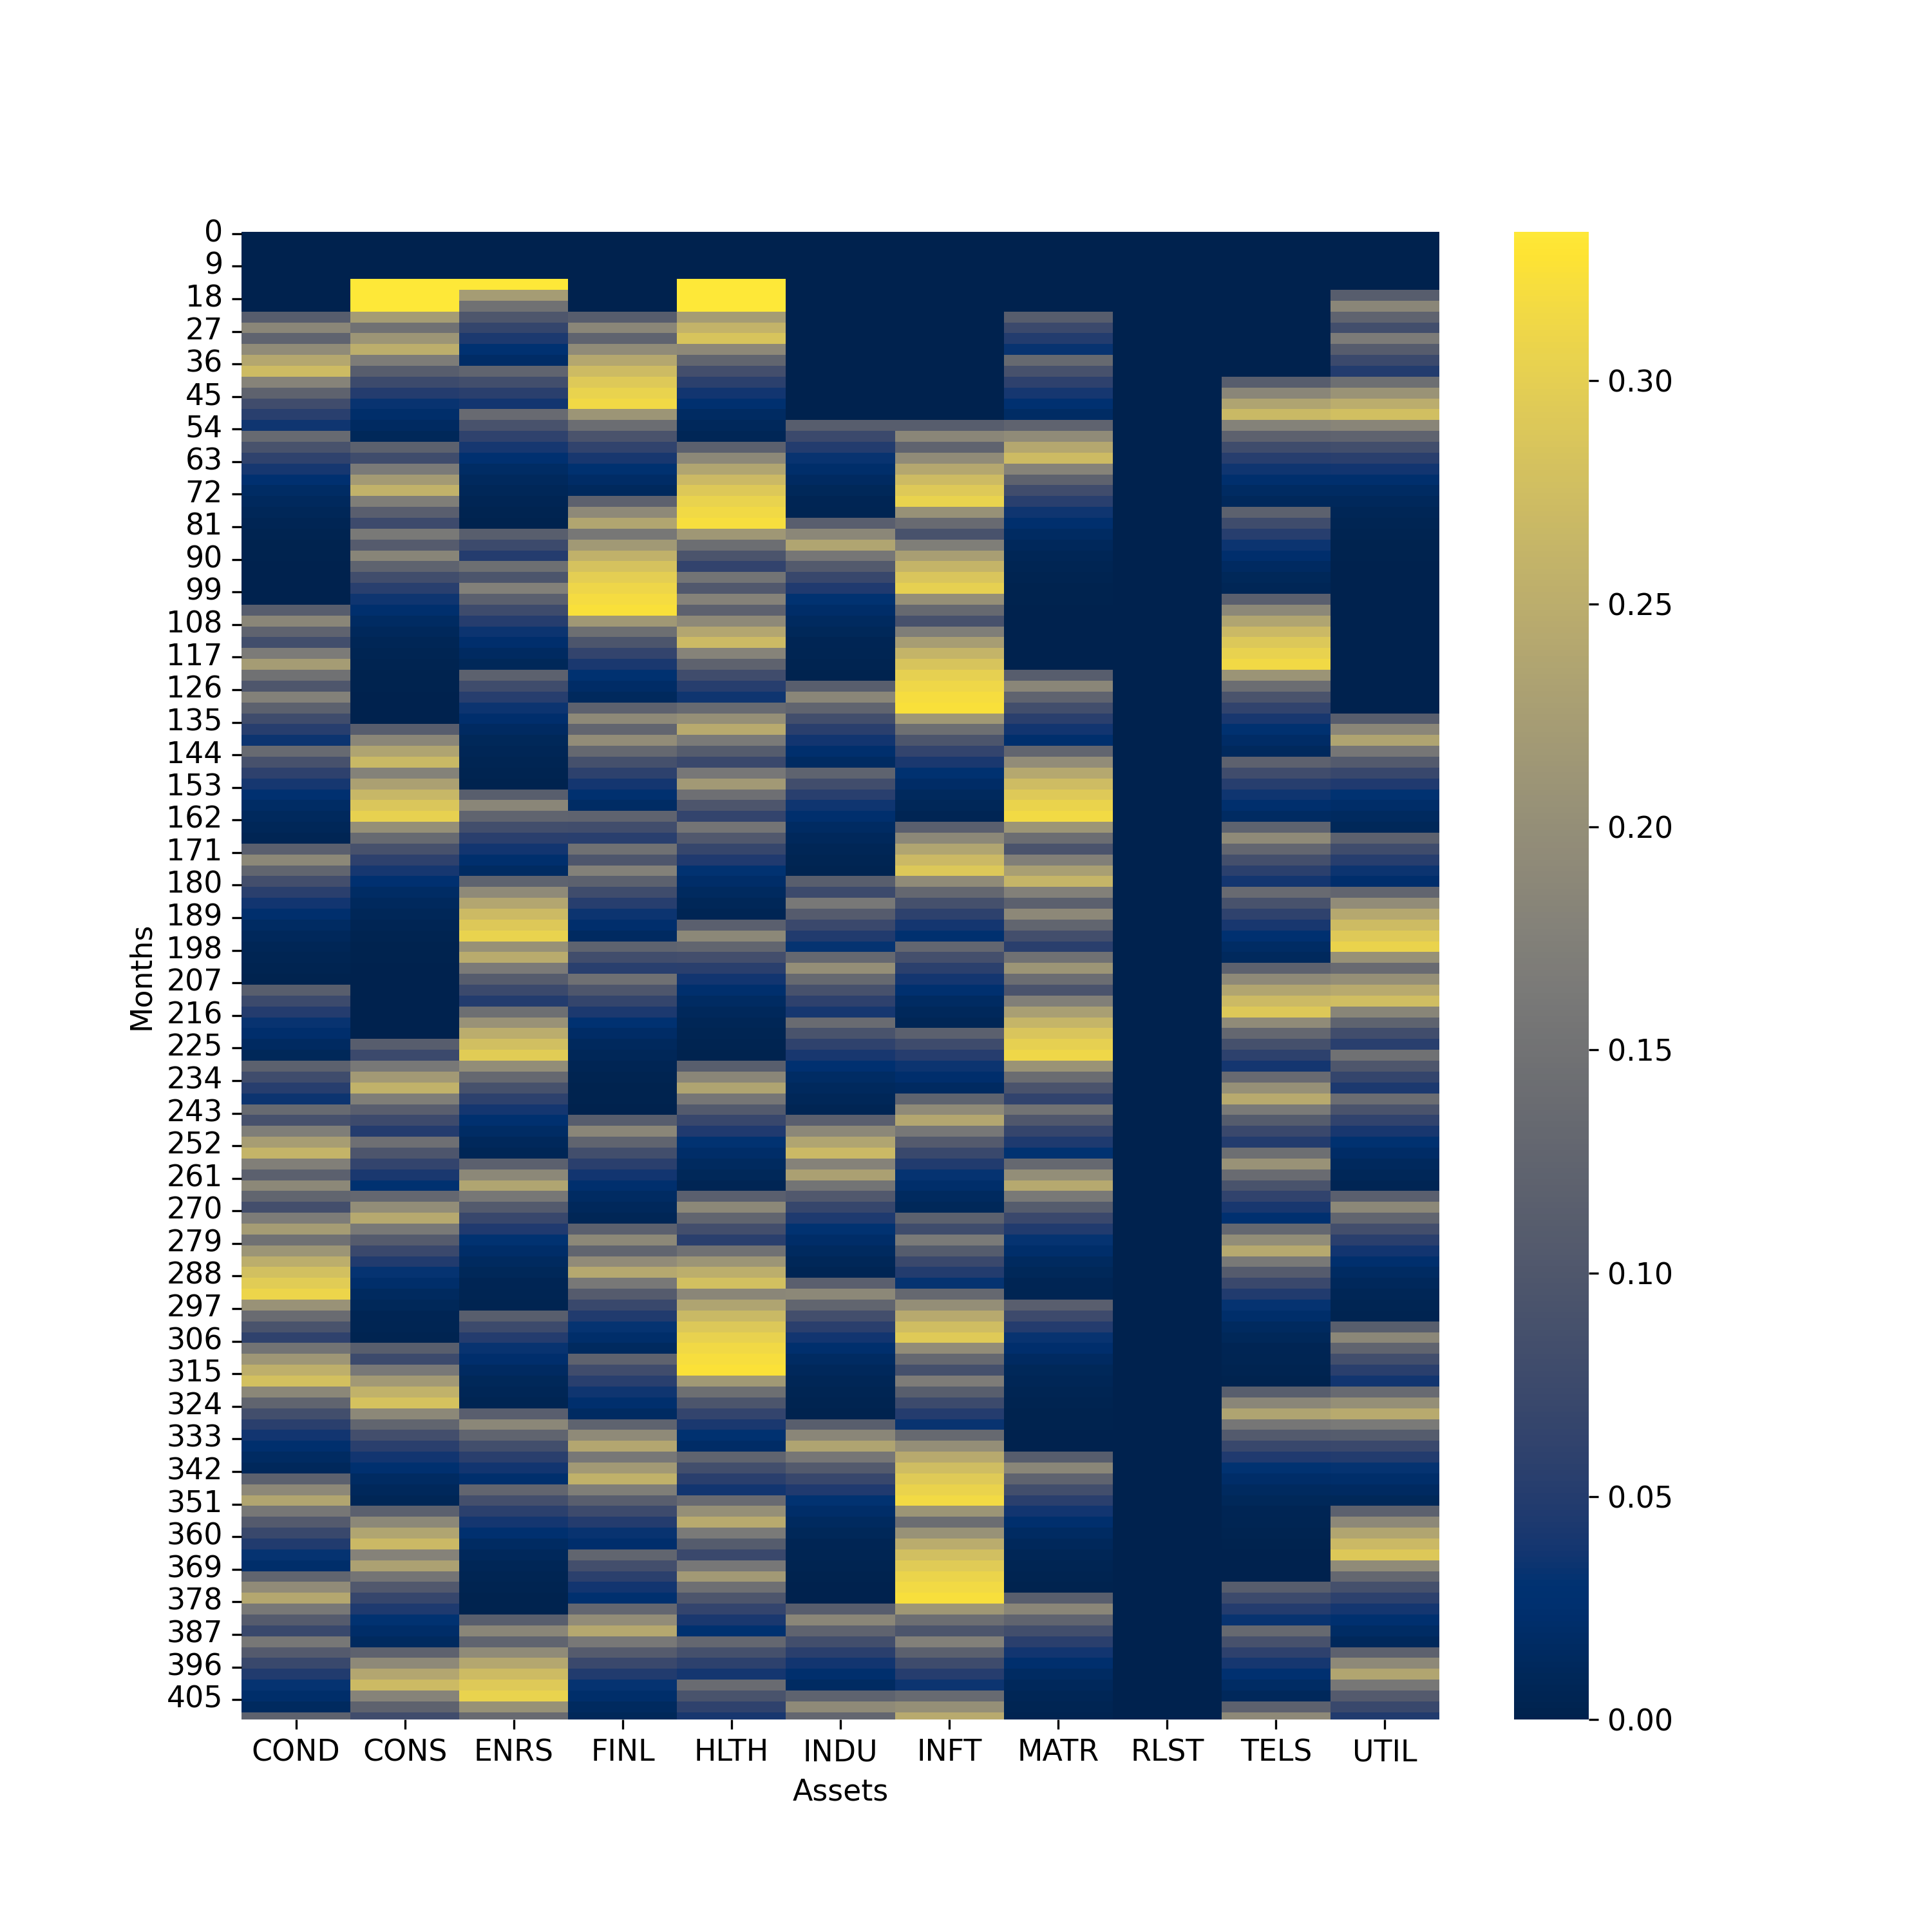
\includegraphics[width=1\textwidth]{Plots/strategy_weights_long_Sectors.png}}
\end{figure} 

\begin{figure}[H]
           \captionsetup{justification=centering}
   \caption{Monthly Weights for Long only Industry Group Momentum Portfolios}
    \label{fig_11}
    \textit{Figure \ref{fig_11}} displays monthly weights for long only industry group momentum portfolios with a holding period of 3 months and a lookback period of 9 months whereby the monthly rebalanced portfolio takes long positions in the 3 best performing industry groups of the market-weighted S\&P500. The figure shows results for the period between September 1989 to October 2023. Different colors represent weight levels.
    \centerline{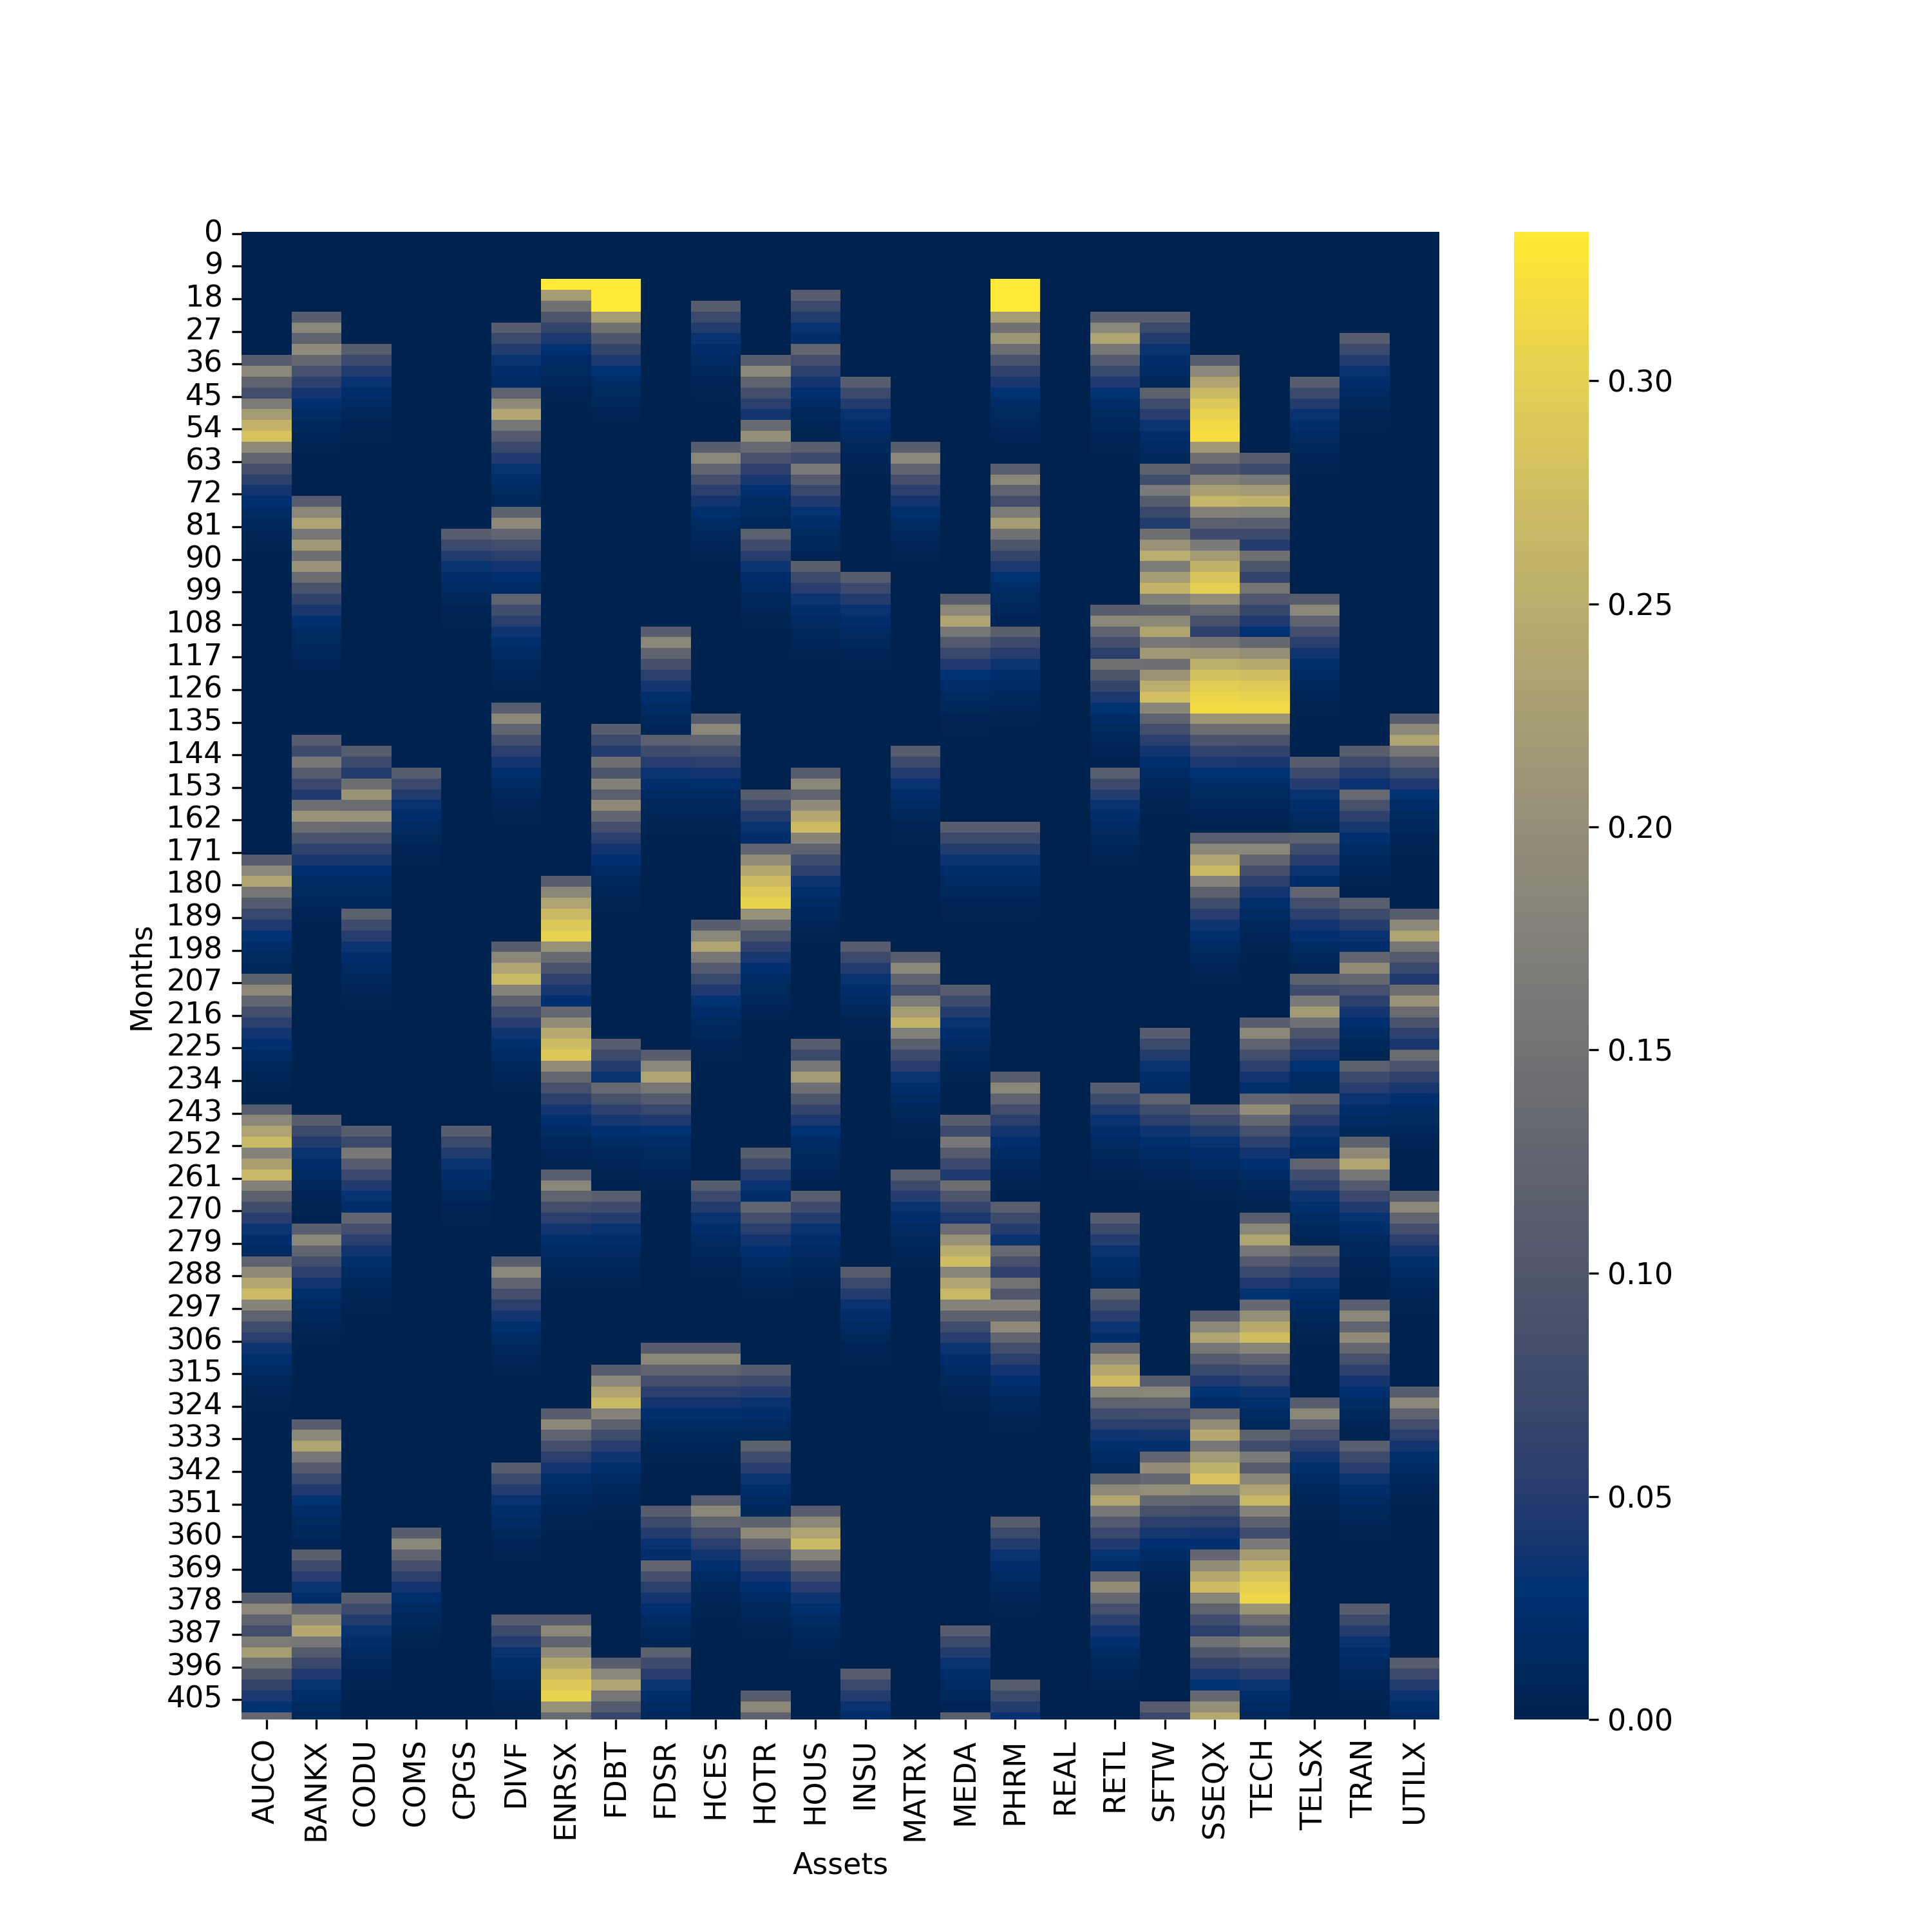
\includegraphics[width=1\textwidth]{Plots/strategy_weights_long_IG.png}}
\end{figure} 

\begin{figure}[H]
           \captionsetup{justification=centering}
   \caption{Monthly Weights for Long/Short Sector Momentum Portfolios}
    \label{fig_12}
    \textit{Figure \ref{fig_12}} displays monthly weights for long/short sector momentum portfolios with a holding period of 3 months and a lookback period of 9 months whereby the monthly rebalanced portfolio takes long (short) positions in the 3 best (worst) performing sectors of the market-weighted S\&P500. The figure shows results for the period between September 1989 to October 2023. Different colors represent weight levels.
    \centerline{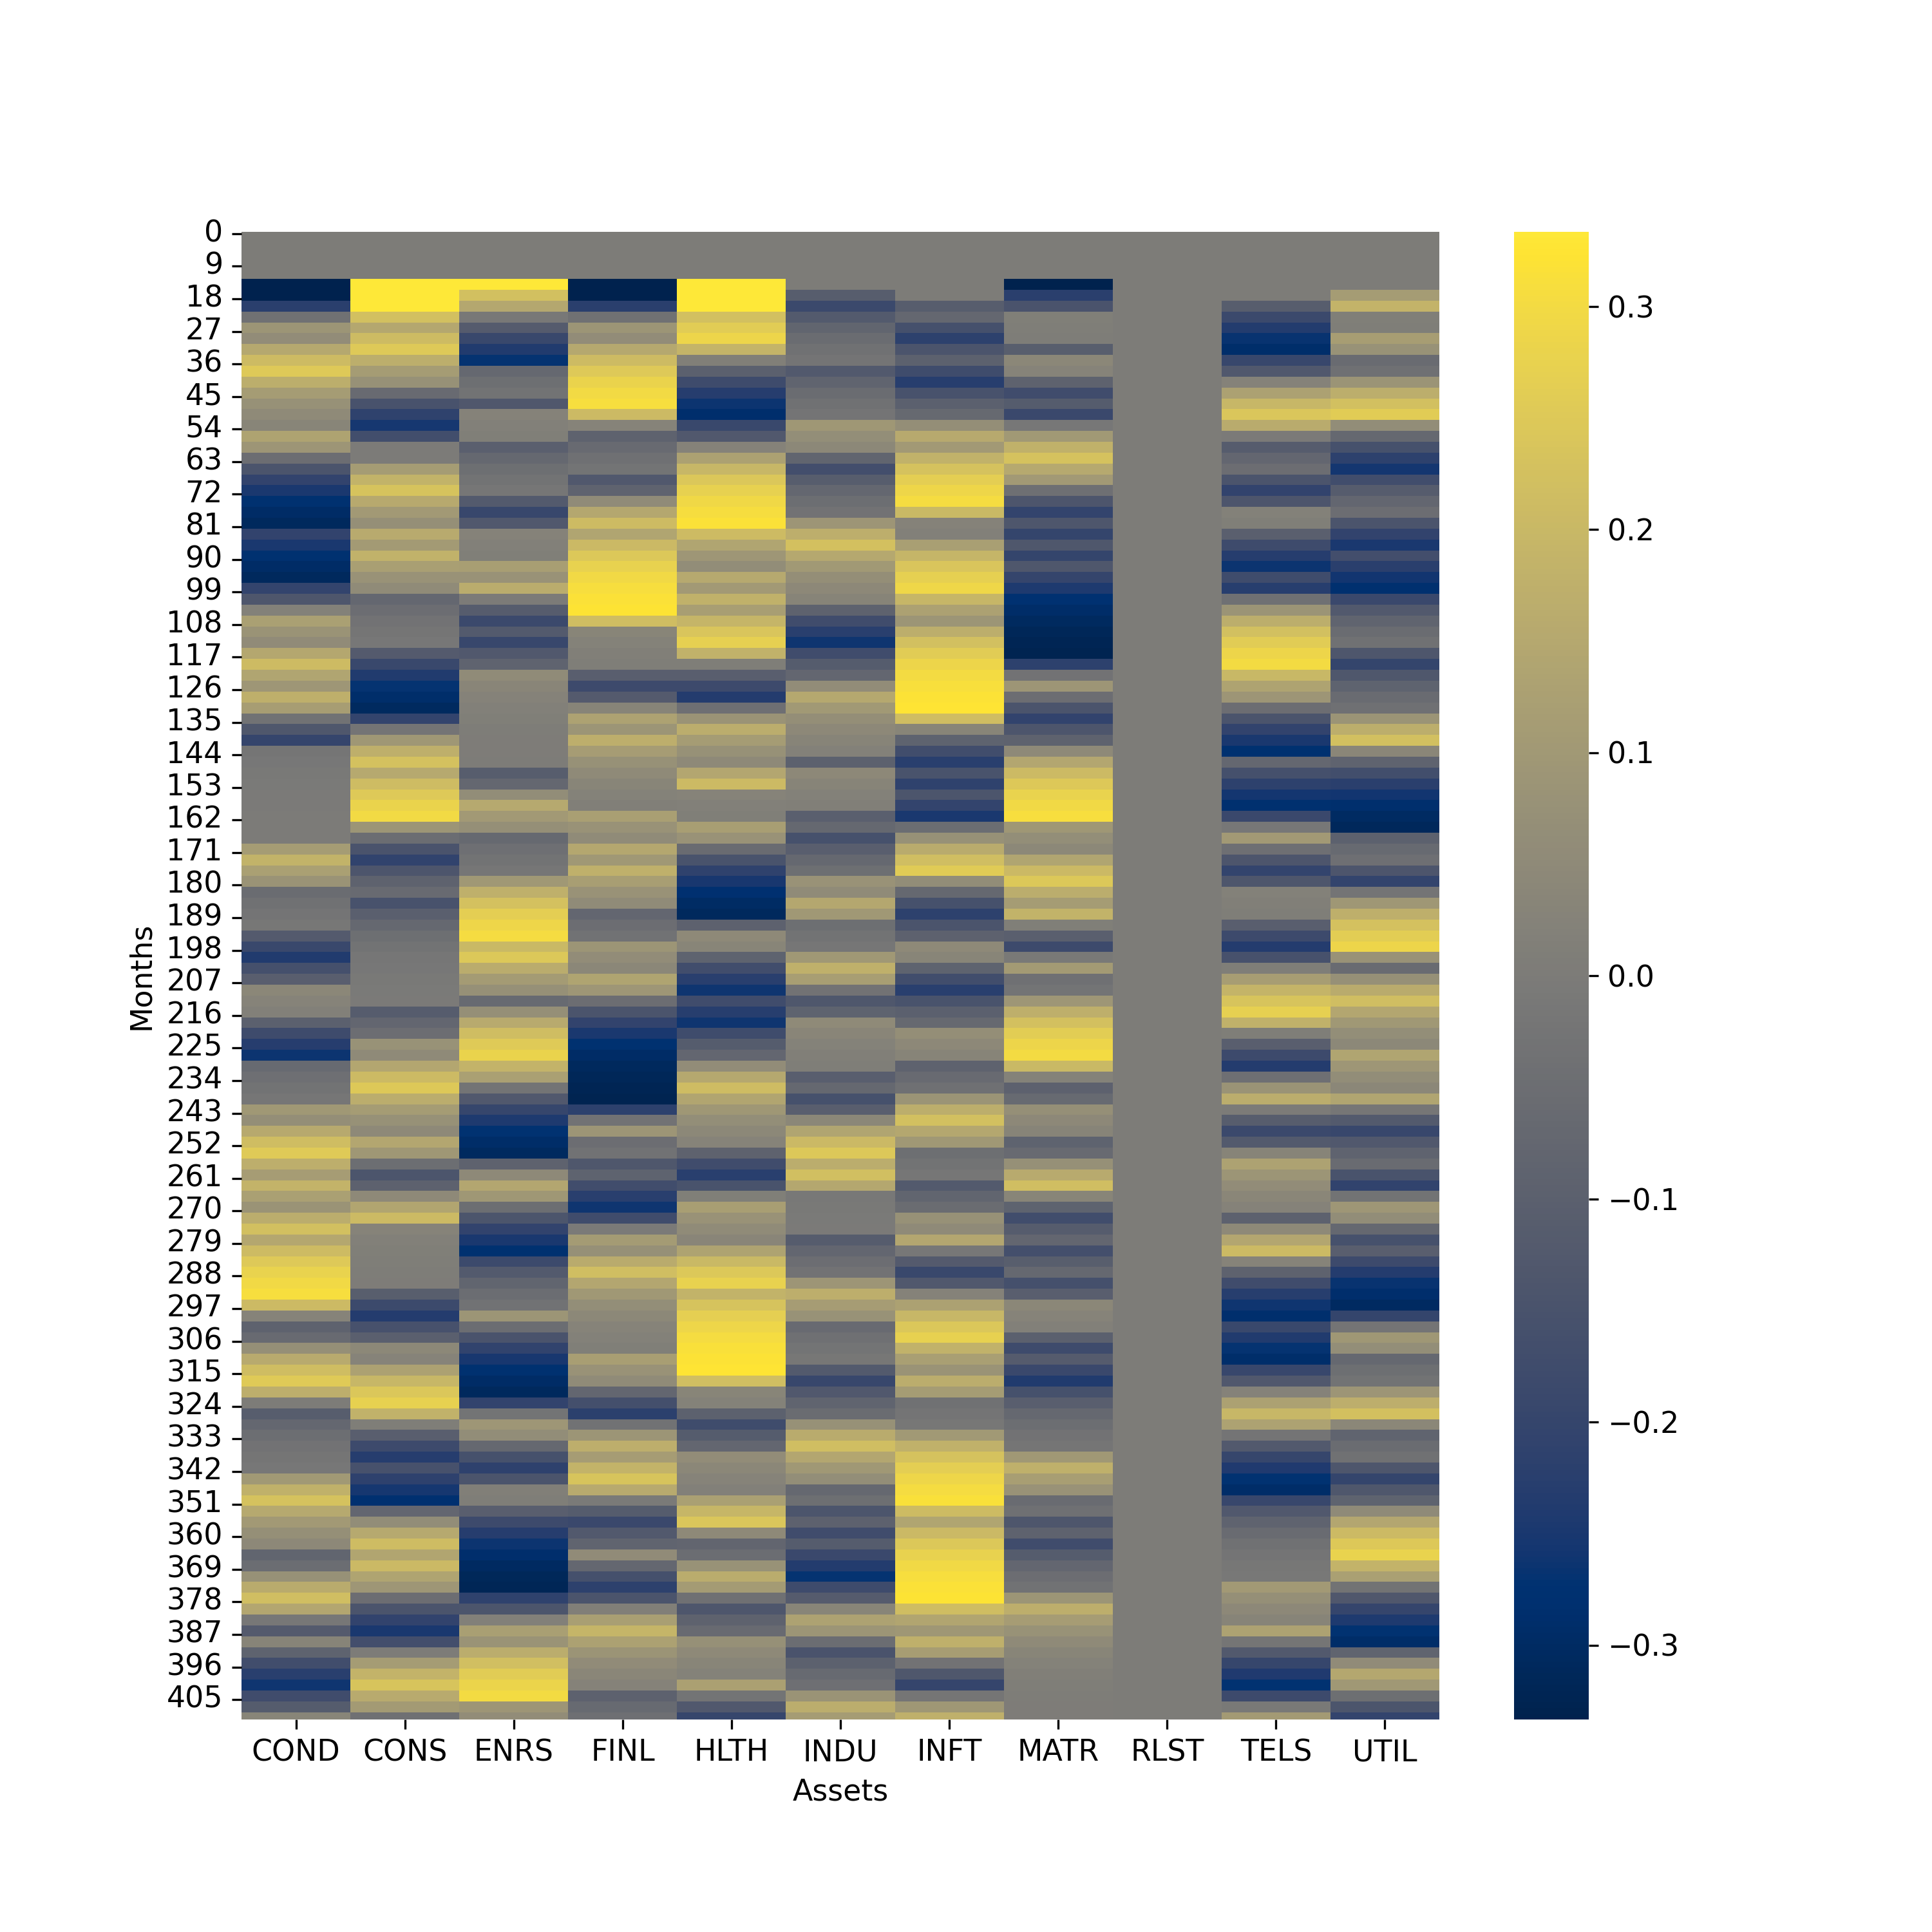
\includegraphics[width=1\textwidth]{Plots/strategy_weights_long_short_Sectors.png}}
\end{figure}

\begin{figure}[H]
           \captionsetup{justification=centering}
   \caption{Monthly Weights for Long/Short Industry Group Momentum Portfolios}
    \label{fig_13}
    \textit{Figure \ref{fig_13}} displays monthly weights for long/short industry group momentum portfolios with a holding period of 3 months and a lookback period of 9 months whereby the monthly rebalanced portfolio takes long (short) positions in the 3 best (worst) performing industry groups of the market-weighted S\&P500. The figure shows results for the period between September 1989 to October 2023. Different colors represent weight levels.
    \centerline{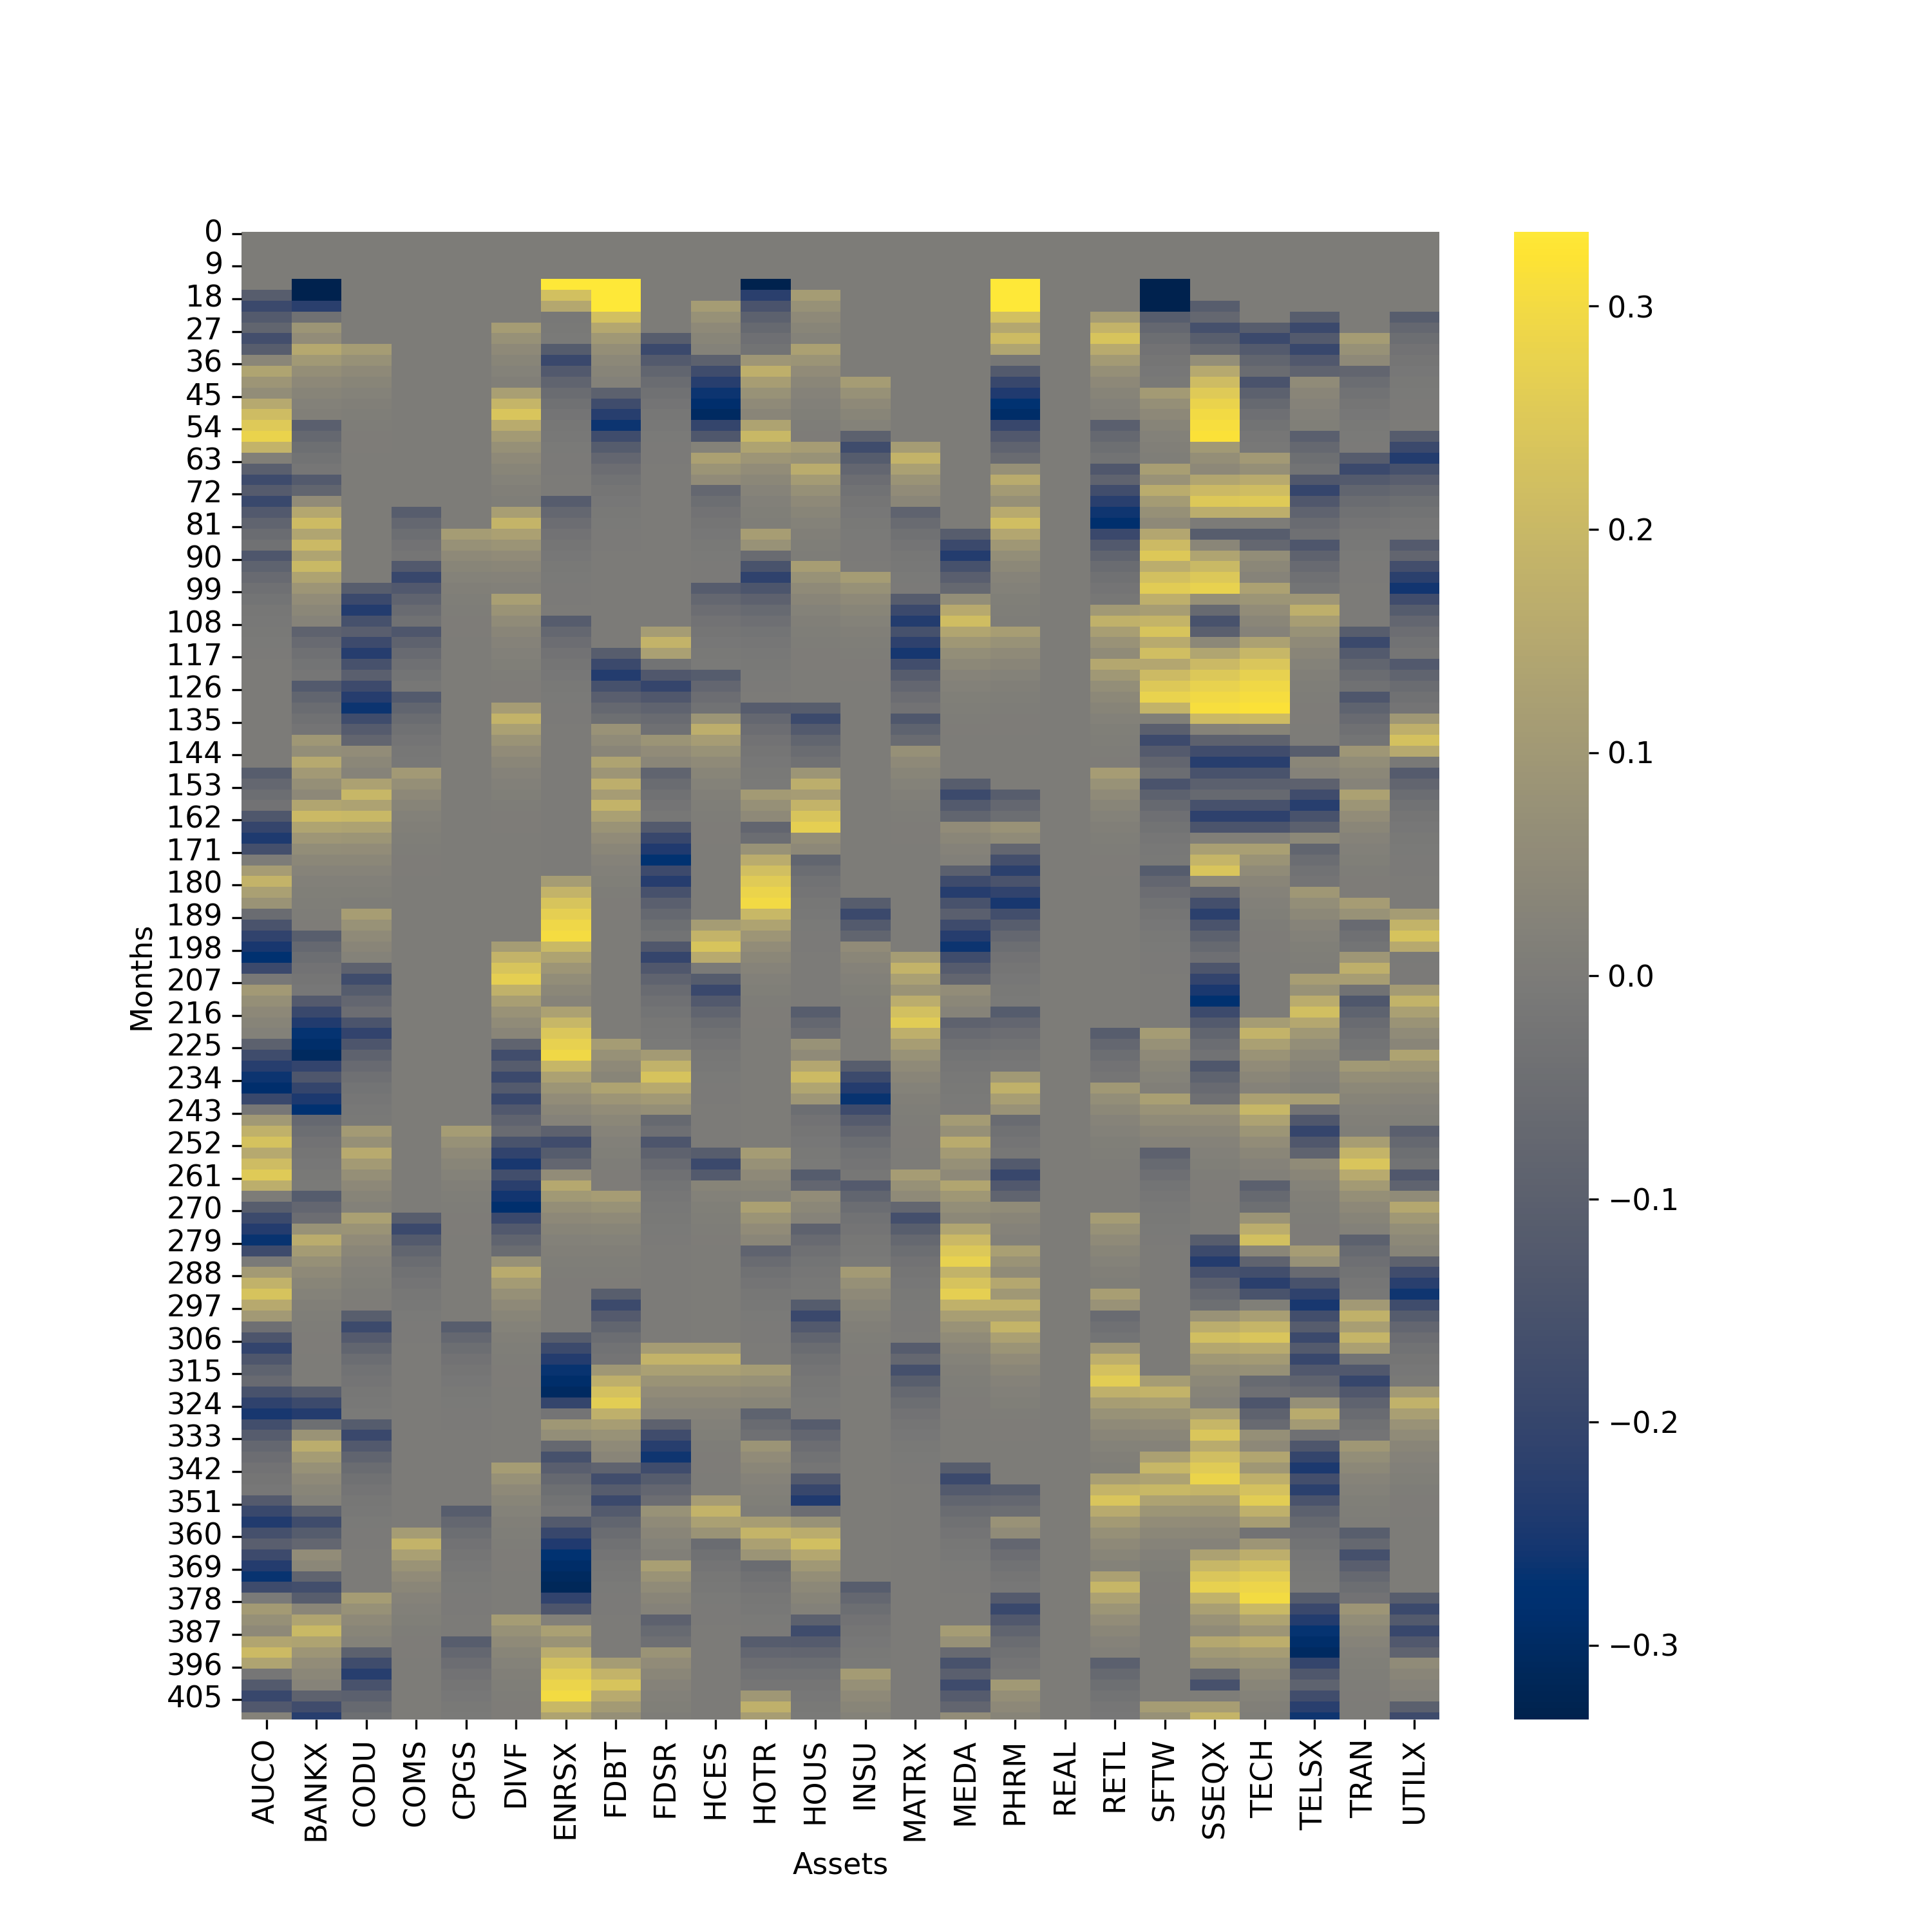
\includegraphics[width=1\textwidth]{Plots/strategy_weights_long_short_IG.png}}
\end{figure} 

\end{document}
